\documentclass[12pt]{article}
% Load packages
\usepackage{url}  % Formatting web addresses  
\usepackage{ifthen}  % Conditional 
\usepackage{multicol}   %Columns
\usepackage[utf8]{inputenc} %unicode support
\usepackage{amsmath}
\usepackage{amssymb}
\usepackage{epsfig}
\usepackage{epstopdf}
\usepackage{graphicx}
\usepackage[margin=0.1pt,font=footnotesize,labelfont=bf]{caption}
\usepackage{setspace}
%\usepackage{longtable}
\usepackage{colortbl}
%\usepackage{palatino,lettrine}
%\usepackage{times}
%\usepackage[applemac]{inputenc} %applemac support if unicode package fails
%\usepackage[latin1]{inputenc} %UNIX support if unicode package fails
\usepackage[wide]{sidecap}
%\usepackage[authoryear,round,comma,sort&compress]{natbib}
\usepackage[square,sort&compress,comma,numbers]{natbib}
%\usepackage[authoryear,round]{natbib}
\usepackage{supertabular}
\usepackage{simplemargins}
\usepackage{comment}
\usepackage{lineno}

\urlstyle{rm}

%\textwidth = 6.50 in
%\textheight = 9.5 in
%\oddsidemargin =  0.0 in
%\evensidemargin = 0.0 in
%\topmargin = -0.50 in
%\headheight = 0.0 in
%\headsep = 0.25 in
%\parskip = 0.15in
%\linespread{1.75}
\doublespace

%\usepackage{geometry}
\usepackage{fullpage}

%\bibliographystyle{plain}
\bibliographystyle{plos2009}

\makeatletter
\renewcommand\subsection{\@startsection
	{subsection}{2}{0mm}
	{-0.05in}
	{-0.5\baselineskip}
	{\normalfont\normalsize\bfseries}}
\renewcommand\subsubsection{\@startsection
	{subsubsection}{2}{0mm}
	{-0.05in}
	{-0.5\baselineskip}
	{\normalfont\normalsize\itshape}}
\renewcommand\section{\@startsection
	{subsection}{2}{0mm}
	{-0.2in}
	{0.05\baselineskip}
	{\normalfont\large\bfseries}}	
\renewcommand\paragraph{\@startsection
	{paragraph}{2}{0mm}
	{-0.05in}
	{-0.5\baselineskip}
	{\normalfont\normalsize\itshape}}
\makeatother

%Review style settings
%\newenvironment{bmcformat}{\begin{raggedright}\baselineskip20pt\sloppy\setboolean{publ}{false}}{\end{raggedright}\baselineskip20pt\sloppy}

%Publication style settings

% Single space'd bib -
\setlength\bibsep{0pt}

\renewcommand{\rmdefault}{phv}\renewcommand{\sfdefault}{phv}
\newcommand{\norm}[1]{\left\lVert#1\right\rVert}

% Change the number format in the ref list -
\renewcommand{\bibnumfmt}[1]{#1.}

% Change Figure to Fig.
\renewcommand{\figurename}{Fig.}

% Begin ...
\begin{document}
\begin{titlepage}
{\par\centering\textbf{\Large Dynamic Modeling of Cell-Free Biochemical Networks using Effective Kinetic Models}}
\vspace{0.05in}
{\par \centering \large{Joseph A. Wayman, Adithya Sagar and Jeffrey D. Varner$^{*}$}}
\vspace{0.10in}
{\par \centering \large{School of Chemical and Biomolecular Engineering}}
{\par \centering \large{Cornell University, Ithaca NY 14853}}
\vspace{0.1in}
{\par \centering \textbf{Running Title:}~Effective models of metabolism}
\vspace{0.1in}
{\par \centering \textbf{To be submitted:}~\textit{Processes}}
\vspace{0.5in}
{\par \centering $^{*}$Corresponding author:}
{\par \centering Jeffrey D. Varner,}
{\par \centering Associate Professor, School of Chemical and Biomolecular Engineering,}
{\par \centering 244 Olin Hall, Cornell University, Ithaca NY, 14853} 
{\par \centering Email: jdv27@cornell.edu} 
{\par \centering Phone: (607) 255 - 4258}
{\par \centering Fax: (607) 255 - 9166}
\end{titlepage}
\date{}
\thispagestyle{empty}
\pagebreak
%%%%%%%%%%%%%%%%%%%%%%%%%%%%%%%%%%%%%%%%%%%%%%%%%%%%%%%%%%%%%%%%%%%%%%%%%%%%%%%%%%%%%%%%%%%%%%%%%%%%%%%%%%%
%%%%%%%%%%%%%%%%%%%%%%%%%%%%%%%%%%%%%%%%%%%%%%%%%%%%%%%%%%%%%%%%%%%%%%%%%%%%%%%%%%%%%%%%%%%%%%%%%%%%%%%%%%%
\section*{Abstract}
Cell-free systems offer many advantages for the study, manipulation and modeling of metabolism compared to \textit{in vivo} processes.
Many of the challenges confronting genome-scale kinetic modeling can potentially be overcome in a cell-free system. 
For example, there is no complex transcriptional regulation to consider, transient metabolic measurements are easier to obtain, and we no longer have to consider cell growth. 
Thus, cell-free operation holds several significant advantages for model development, identification and validation. 
Theoretically, genome-scale cell-free kinetic models may be possible for industrially important organisms, such as \textit{E. coli}, if a simple, tractable framework for integrating allosteric regulation with enzyme kinetics can be formulated. 
Toward this unmet need, we present an effective biochemical network modeling framework for building dynamic cell-free metabolic models.
The key innovation of our approach is the integration of simple effective rules encoding complex allosteric regulation with traditional kinetic pathway modeling. 
We tested our approach by modeling the time evolution of several hypothetical cell-free metabolic networks. 
We found that simple effective rules, when integrated with traditional enzyme kinetic expressions, captured complex allosteric patterns such as ultrasensitivity or non-competitive inhibition in the absence of mechanistic information. 
Second, when integrated into network models, these rules captured classic regulatory patterns such as product-induced feedback inhibition. 
Lastly, we showed, at least for the network architectures considered here, that we could simultaneously estimate kinetic parameters and allosteric connectivity from synthetic data. 
While only an initial proof-of-concept, the framework presented here could be an important first step toward genome-scale cell-free kinetic modeling of the biosynthetic capacity of industrially important organisms.

{\noindent \textbf{Keywords:}~Cell-free metabolism, Mathematical modeling}

\pagebreak

\setcounter{page}{1}

\linenumbers

\section*{Introduction}
Mathematical modeling has long contributed to our understanding of metabolism. 
Decades before the genomics revolution, mechanistically, structured metabolic models arose from the desire to predict microbial phenotypes resulting from changes in intracellular or extracellular states \citep{1976_fredrickson_BiotechBioeng}. 
The single cell \textit{E. coli} models of Shuler and coworkers pioneered the construction of large-scale, dynamic metabolic models that incorporated multiple, regulated catabolic and anabolic pathways constrained by experimentally determined kinetic parameters \citep{1984_domach_shuler_BiotechBioeng_01}. 
Shuler and coworkers generated many single cell kinetic models, including single cell models of eukaryotes \citep{1989_steinmeyer_shuler_ChemEngSci,1992_wu_shuler_AnnNYAcadSci}, minimal cell architectures \citep{2004_castellanos_shuler_PNAS}, as well as DNA sequence based whole-cell models of \textit{E. coli} \citep{2008_atlas_shuler_IETSysBio}.
Conversely, highly abstracted kinetic frameworks, such as the cybernetic framework, represented a paradigm shift, viewing cells as growth-optimizing strategists \citep{1985_dhurjati_ramkrishna_tsao_BiotechBioeng}. 
Cybernetic models have been highly successful at predicting metabolic choice behavior, e.g., diauxie behavior \citep{1986_kompala_ramkrishna_tsao_BiotechBioeng}, steady-state multiplicity \citep{2012_kim_ramkrishna_BiotechProg}, as well as the cellular response to metabolic engineering modifications \citep{1999_varner_ramkrishna_MetaEng}. 
Unfortunately, traditional, fully structured cybernetic models also suffer from an identifiability challenge, as both the kinetic parameters and an abstracted model of cellular objectives must be estimated simultaneously. 
Recent cybernetic formulations from Ramkrishna and colleagues have successfully treated this identifiability challenge through elementary mode reduction, though the techniques replace detailed biological mechanism with an optimization heuristic \cite{2009_song_ramkrishna_BiotechBioeng,Song:2011aa}. 

In the post genomics world, large-scale stoichiometric reconstructions of microbial metabolism popularized by static, constraint-based modeling techniques such as flux balance analysis (FBA) have become standard tools \citep{2012_lewis_palsson_NatRevMicrobio}. 
Since the first genome-scale stoichiometric model of \textit{E. coli}, developed by Edwards and Palsson \citep{2000_edwards_palsson_PNAS}, well over 100 organisms, including industrially important prokaryotes such as \textit{E. coli} \citep{Feist:2007aa} or \textit{B. subtilis} \citep{Oh:2007aa}, are now available \citep{2009_feist_palsson_NatRevMicrobio}. 
Stoichiometric models rely on a pseudo-steady-state assumption to reduce unidentifiable genome-scale kinetic models to an underdetermined linear algebraic system, which can be solved efficiently even for large systems.  
Traditionally, stoichiometric models have also neglected explicit descriptions of metabolic regulation and control mechanisms, instead opting to describe the choice of pathways by prescribing an objective function on metabolism. 
Interestingly, similar to early cybernetic models, the most common metabolic objective function has been the optimization of biomass formation \citep{2002_ibarra_edwards_palsson_Nat}, although other metabolic objectives have also been estimated \citep{2007_schuetz_sauer_MolSysBio}. 
Recent advances in constraint-based modeling have overcome the early shortcomings of the platform, including capturing metabolic regulation and control \citep{2013_hyduke_lewis_palsson_MolBioSys}. 
Thus, modern constraint-based approaches have proven extremely useful in the discovery of metabolic engineering strategies and represent the state of the art in metabolic modeling \citep{2013_mccloskey_palsson_feist_MolSysBio, 2012_zomorrodi_maranas_MetaEng}. However, genome-scale kinetic models of industrial important organisms such as \textit{E. coli} have yet to be constructed. 

Cell-free systems offer many advantages for the study, manipulation and modeling of metabolism compared to \textit{in vivo} processes.
Central amongst these advantages is direct access to metabolites and the microbial biosynthetic machinery without the interference of a cell wall. 
This allows us to control as well as interrogate the chemical environment while the biosynthetic machinery is operating, potentially at a fine time resolution.
Second, cell-free systems also allow us to study biological processes without the complications associated with cell growth.
Cell-free protein synthesis (CFPS) systems are arguably the most prominent examples of cell-free systems used today \citep{Jewett:2008aa}. 
However, CFPS is not new; CFPS in crude \textit{E. coli} extracts has been used since the 1960s to explore fundamentally important biological mechanisms \citep{MATTHAEI:1961aa,NIRENBERG:1961aa}. 
Today, cell-free systems are used in a variety of applications ranging from therapeutic protein production \citep{Lu:2014aa} to synthetic biology \citep{Hodgman:2012aa}. 
Interestingly, many of the challenges confronting genome-scale kinetic modeling can potentially be overcome in a cell-free system. 
For example, there is no complex transcriptional regulation to consider, transient metabolic measurements are easier to obtain, and we no longer have to consider cell growth. 
Thus, cell-free operation holds several significant advantages for model development, identification and validation.
Theoretically, genome-scale cell-free kinetic models may be possible for industrially important organisms, such as \textit{E. coli} or \textit{B. subtilis}, if a simple, tractable framework for integrating allosteric regulation with enzyme kinetics can be formulated. 

In this study, we present an effective biochemical network modeling framework for building dynamic cell-free metabolic models.
The key innovation of our approach is the seamless integration of simple effective rules encoding complex regulation with traditional kinetic pathway modeling. 
This integration allows the description of complex regulatory interactions, such as time-dependent allosteric regulation of enzyme activity, in the absence of specific mechanistic information. 
The regulatory rules are easy to understand, easy to formulate and do not rely on overarching theoretical abstractions or restrictive assumptions. 
We tested our approach by modeling the time evolution of several hypothetical cell-free metabolic networks. 
In particular, we tested whether our effective modeling approach could describe classically expected enzyme kinetic behavior, and second whether we could simultaneously estimate kinetic parameters and regulatory connectivity, in the absence of specific mechanistic knowledge, from synthetic experimental data. 
Toward these questions, we explored five hypothetical cell-free networks. 
Each network shared the same enzymatic connectivity, but had different allosteric regulatory connectivity. 
We found that simple effective rules, when integrated with traditional enzyme kinetic expressions, captured complex allosteric patterns such as ultrasensitivity or non-competitive inhibition in the absence of mechanistic information. 
Second, when integrated into network models, these rules captured classical regulatory patterns such as product-induced feedback inhibition. 
Lastly, we showed, at least for the network architectures considered here, that we could simultaneously estimate kinetic parameters and allosteric connectivity from synthetic data. 
While only an initial proof-of-concept, the framework presented here could be an important first step toward genome-scale cell-free kinetic modeling of the biosynthetic capacity of industrially important organisms.

\clearpage

\section*{Results}

\subsection*{Formulation and properties of effective cell-free metabolic models.}
We developed two proof-of-concept metabolic networks to investigate the features of our effective biochemical network modeling approach (Fig. \ref{fig-networks}). 
In both examples, substrate S was converted to the end products P$_{1}$ and P$_{2}$ through a series of enzymatically catalyzed reactions, including a branch point at hypothetical metabolite M$_{2}$. 
Several of these reactions involved cofactor dependence (AH or A), and various allosteric regulatory mechanisms modified the activity of pathway enzymes. 
Network A included feedback inhibition of the initial pathway enzyme ($E_{1}$) by pathway end products P$_{1}$ and P$_{2}$ (Fig. \ref{fig-networks}A). 
On the other hand, network B involved feedback inhibition of $E_{1}$ by P$_{2}$ and $E_{6}$ by P$_{1}$ (Fig. \ref{fig-networks}B). 
In both networks, branch point enzymes $E_{3}$ and $E_{6}$ were subject to feed-forward activation by reduced cofactor AH. 
Lastly, it is known experimentally that cell-free systems have a finite operational lifespan. 
Loss of biosynthetic capability could be a function of many factors, e.g., cofactor or metabolite limitations. 
We modeled the loss of biosynthetic capability as a non-specific first-order decay of enzyme activity.

Allosteric regulation of enzyme activity was modeled by combining individual regulatory contributions to the activity of pathway enzymes into a control coefficient using an integration rule (Fig. \ref{fig-control-schematic}).  
This strategy is similar in spirit to the Constrained Fuzzy Logic (cFL) approach of Lauffenburger and coworkers which has been used to effectively model signal transduction pathways important in human health \citep{Morris:2011aa}. 
In our formulation, Hill-like transfer functions $0 \leq f\left(\mathcal{Z}\right) \leq 1$ were used to calculate the influence of factor abundance upon target enzyme activity. 
In this context, factors can be individual metabolite levels or some function, e.g., the product of metabolite levels. 
However, more generally, factors can also correspond to non-modeled influences, categorial variables or other abstract quantities. 
In the current study, we simply let $\mathcal{Z}$ correspond to the abundance of individual metabolites, however in general this can be a complex function of both modeled and unmodeled factors. 
When an enzyme was potentially sensitive to more than one regulatory input, logical integration rules were used to select which regulatory transfer function influenced enzyme activity at any given time. 
Thus, our test networks involved important features such as cofactor recycling, enzyme activity and metabolite dynamics, as well as multiple overlapping allosteric regulatory mechanisms.  

The rule-based regulatory strategy approximated the behavior of classical allosteric activation and inhibition mechanisms (Fig. \ref{fig-kinetics-simulations}). 
We considered the enzyme catalyzed conversion of substrate S to a product P, where the overall reaction rate was modeled as the product of a Michaelis-Menten term and an effective allosteric control variable reflecting the particular regulatory interaction. 
We first explored feed-forward substrate activation of enzyme activity (for both positive and negative cooperativity). 
Consistent with classical data, the rule-based strategy predicted a sigmoidal relationship between substrate abundance and reaction rate as a function of the cooperativity parameter (Fig. \ref{fig-kinetics-simulations}A). 
For cooperativity parameters less than unity, increased substrate abundance \textit{decreased} the maximum reaction rate. 
This was consistent with the idea that substrate binding \textit{decreased} at regulatory sites, which negatively impacted substrate binding at the active site. 
On the other hand, as the cooperativity parameter increased past unity, the rate of conversion of substrate S to product P by enzyme $E$ approached a step function. 
In the presence of an inhibitor, the rule-based strategy predicted non-competitive like behavior as a function of the cooperativity parameter (Fig. \ref{fig-kinetics-simulations}B). 
When the control gain parameter, $\kappa_{ij}$ in Eqn. \eqref{eqn:control-factor}, was greater than unity, the inhibitory force was directly proportional to the cooperativity parameter, $\eta$ in Eqn. \eqref{eqn:control-factor}. 
Thus, as the cooperativity parameter increased, the maximum reaction rate decreased (Fig. \ref{fig-kinetics-simulations}B). 
Interestingly, our rule-based approach was unable to directly simulate competitive inhibition of enzyme activity. 
Taken together, the rule-based strategy captured classical regulatory patterns for both enzyme activation and inhibition. 
Thus, we are able to model complex kinetic phenomena such as ultrasensitivity, despite an effective description of reaction kinetics. 
    
End product yield was controlled by feedback inhibition, while product selectivity was controlled by branch point enzyme inhibition (Fig. \ref{fig-onoff-simulations}). 
A critical test of our modeling approach was to simulate networks with known behavior. 
If we cannot reproduce the expected behavior of simple networks, then our effective modeling strategy, and particularly the rule-based approximation of allosteric regulation, will not be feasible for genome-scale cell-free problems. We considered two cases, control ON/OFF, for each network configuration. 
Each of these cases had identical kinetic parameters and initial conditions; the \textit{only} differences between the cases were the allosteric regulation rules and the control parameters associated with these rules. 
As expected, end product accumulation was larger for network A when the control was OFF (no feedback inhibition of $E_{1}$ by P$_{1}$ and P$_{2}$),
as compared to the ON case (Fig. \ref{fig-onoff-simulations}A). 
We found this behavior was robust to the choice of underlying kinetic parameters, as we observed that same qualitative response across an ensemble of 100 randomized parameter sets, for fixed control parameters. 
The control ON/OFF response of network B was more subtle. 
In the OFF case, the behavior was qualitatively similar to network A. 
However, for the ON case, flux was diverted away from P$_{2}$ formation by feedback inhibition of $E_{6}$ activity at the M$_{2}$ branch point by P$_{1}$ (Fig. \ref{fig-onoff-simulations}B). 
Lower $E_{6}$ activity at the M$_{2}$ branch point allowed more flux toward P$_{1}$ formation, hence the yield of P$_{1}$ also increased (Fig. \ref{fig-onoff-simulations}C). 
Again, the control ON/OFF behavior of network B was robust to changes in kinetic parameters, as the same qualitative trend was conserved across an ensemble of 100 randomized parameters, for fixed control parameters. 
Taken together, these simulations suggested that the rule-based allosteric control concept could robustly capture expected feedback behavior for networks with uncertain kinetic parameters.

\subsection*{Estimating parameters and effective allosteric regulatory structures.}
A critical challenge for any dynamic model is the estimation of kinetic parameters. 
For metabolic processes, there is also the added challenge of identifying the regulation and control structures that manage metabolism. 
Of course, these issues are not independent; any description of enzyme activity regulation will be a function of system state, which in turn depends upon the kinetic parameters. 
For cell free systems, regulated gene expression has been removed, however, enzyme activity regulation is still operational. 
We explored this linkage by estimating model parameters from synthetic data using both network structures. 
We generated synthetic measurements of the substrate S, intermediate M$_{5}$ and end product P$_1$ approximately every 20 min using
network A. This data set is similar to published cell free studies both in terms of network coverage, and sampling frequency \citep{Jewett:2008aa}. 
We then generated an ensemble of model parameter estimates by minimizing the difference between model simulations and the synthetic data using particle swarm optimization (PSO), starting from random initial parameter guesses. The estimation of kinetic parameters was sensitive to the choice of regulatory structure (Fig. \ref{fig-parameter-fit}). 
PSO identified an ensemble of parameters that bracketed the mean of the synthetic measurements in less than 1000 iterations when the control structure was correct (Fig. \ref{fig-parameter-fit}A and B). 
However, with control mismatch (network B simulated with network A parameters), model simulations were not consistent with the synthetic data  (Fig. \ref{fig-parameter-fit}C and D). 
Taken together, these results suggested that we could perhaps simultaneously estimate both parameters and network control architectures, as incorrect control structures would be manifest as poor model fits.

We modified our particle swarm identification strategy to simultaneously search over both kinetic parameters and putative control structures. 
In addition to our initial networks, we constructed three additional presumptive network models, each with the same enzymatic connectivity but different allosteric regulation of the pathway enzymes (Fig. \ref{fig-alternative-networks}). 
We then initialized a population of particles, each with one of the five potential regulatory programs and randomized kinetic parameters. 
Thus, we generated an initial population of particles that had \textit{both} different kinetic parameters as well as different control structures. 
We biased the distribution of the particle population according to our \textit{a prior} belief of the correct regulatory program. 
To this end, we considered three different priors, a uniform distribution where each putative regulatory structure represented 20\% of the population and two mixed distributions that were either positively or negatively biased towards the correct structure (network A). 
In both the positively biased and uniform cases the PSO clearly differentiated between the true or closely related structures and those that were materially different (Fig. \ref{fig-control-search}). 
As expected, the positively biased population (40\% of the initial particle population seeded with network A) gave the best results, where the correct structure was preferentially identified (Fig. \ref{fig-control-search}A). 
On the other hand, when given a uniform distribution, the PSO approach identified a combination of network A and network C as the most likely control structures (Fig. \ref{fig-control-search}B). 
Network A and C differ by the regulatory connection between the end product P$_2$ and enzyme $E_{1}$; in network A, end product P$_{2}$ was assumed to inhibit $E_{1}$, while in network C, end product P$_{2}$ activated $E_{1}$.  
Lastly, when the initial population was biased towards incorrect structures (initial population seeded with 90\% incorrect structures), the particle swarm \textit{misidentified} the correct allosteric structure (Fig. \ref{fig-control-search}C). 
Interestingly, while each particle swarm identified parameter sets that minimized the simulation error, the estimated parameter values were not necessarily similar to the true parameters. 
The angle between the estimated and true parameters was not consistently small across the swarms (identical parameters would give an angle of zero). 
This suggested that our particle swarm approach identified a \textit{sloppy} ensemble, i.e., parameter estimates that were individually incorrect but collectively exhibited the correct model behavior.  

We calculated control program output and scaled metabolic flux for the positively, uniformly and negatively biased particle swarms (Fig. \ref{fig-flux-pattern}). 
Network A and network C models from the positively (Fig. \ref{fig-flux-pattern}A) and uniformly (Fig. \ref{fig-flux-pattern}B) biased particle swarms showed similar operational patterns, despite differences in kinetic parameters and control structures.
While models from the negatively biased population had error values similar to the correct structures in the previous swarms, they have different flux and control profiles (Fig. \ref{fig-flux-pattern}C). 
In all cases, regardless of network configuration or parameter values, the rate of enzyme decay was small compared to the other fluxes, and all networks had qualitatively similar trends for $E_{3}$ and $E_{6}$ control. 
Moreover, consistent with the correct model structure, production of end product P$_1$ was the preferred branch for all model configurations. 
However, there was variability in P$_{2}$ production flux across the population of models, especially for the uniform swarm when compared with the other cases. 
High P$_{1}$ branch flux resulted in end product inhibition of $E_{1}$ in both network A and network C, however in network D and E, high P$_1$ flux induced $E_1$ activation. 
These trends were manifested in different flux profiles, where the negatively biased population appeared more uniform across the population compared with the other swarms, and had higher $E_{1}$ specific activity. 
Interestingly, the behavior of network A and network C highlighted an artifact of our integration rule; both a positive or negative feedback connection from P$_2$ to $E_{1}$ were ignored because the P$_{1}$ inhibition of $E_{1}$ dominated. Thus, while theoretically distinct, network A and network C appeared operationally to the PSO algorithm to be the same network. 
On the other hand, networks B, D and E showed distinct behavior that was not consistent with the true network. 
These architectures exhibited either limited inhibition (network B) or activation (network D and E) of $E_{1}$ activity, resulting in significantly different metabolic flux profiles. 
However, the PSO was able to find low error parameter solutions, despite the mismatch in the control structures (error values similar, but not better than the best network A and network C estimates). 
Taken together, these results suggested that a uniform sampling approach could potentially yield an unbiassed estimate of both kinetic parameters and control structures. 
However, the negatively biased particle swarm results illustrated a potential shortcoming of the approach, namely convergence to a local error minimum despite a significantly incorrect control structure. 
This suggested that estimated model structures will need to be further evaluated, for example by generating falsifiable experimental designs which could distinguish between low error solutions.

\clearpage

\section*{Discussion}
In this study, we presented an effective kinetic modeling strategy to dynamically simulate cell-free biochemical networks. 
Our proposed strategy integrated traditional kinetic modeling with an effective rules based approach to dynamically describe metabolic regulation and control. 
We tested this approach by developing kinetic models of hypothetical cell-free metabolic networks. 
In particular, we tested whether our effective modeling approach could describe classically expected behavior, and second whether we could simultaneously estimate kinetic parameters and regulatory connectivity, in the absence of specific mechanistic knowledge, from synthetic experimental data. 
Toward these questions, we explored five hypothetical cell-free networks. 
In each network, a substrate S was converted to the end products P$_{1}$ and P$_{2}$ through a series of enzymatically catalyzed reactions, including a branch point at a hypothetical metabolite M$_{2}$. 
Each network also included the same cofactors and cofactor recycle architecture. 
However, while all five networks shared the same enzymatic connectivity, each had different allosteric regulatory connectivity. 
We found that simple effective rules, when integrated with traditional enzyme kinetic expressions, could capture complex allosteric patterns such as ultrasensitivity, or non-competitive inhibition in the absence of specific mechanistic information. 
Moreover, when integrated into network models, these rules captured classical regulatory patterns such as product-induced feedback inhibition. 
Lastly, we simultaneously estimated kinetic parameters and discriminated between competing regulatory structures, using synthetic data in combination with a modified particle swarm approach.
If we considered all putative regulatory architectures to be equally likely, we were able to estimate a \textit{sloppy} ensemble of models with the correct architecture and kinetic parameters.

The proposed modeling strategy shares features with other popular techniques, but also has several key differences. 
At its core, our effective modeling approach is similar to regulatory constraint-based methods, and to the cybernetic modeling paradigm developed by Ramkrishna and colleagues.
Covert, Palsson and coworkers drastically improved the predictability of constraint-based approaches by integrating Boolean rules into the calculation of metabolic fluxes \citep{Covert:2001aa}.
If the regulated intracellular flux problem is coupled with time-dependent extracellular balances, these models can predict complex behavior such as diauxie growth or the switch between 
aerobic and anaerobic metabolism. Another important feature of this approach is that it scales with biological complexity. 
For example, Covert \emph{et al.} showed that a genome-scale model of \emph{E.~coli} augmented with a Boolean rule layer, 
correctly predicted approximately 80\% of the outcomes of a high-throughput growth phenotyping experiment in \emph{E. coli}.
Further, they showed that they could learn new biology by iteratively refining the model and its associated rules \citep{Covert:2004aa}. 
However, while regulated flux balance analysis is a powerful technique, it does not easily allow the calculation of time-resolved metabolite abundance. 
Additionally, the Boolean rules which populate the regulatory layer are limited to ON/OFF decisions; for qualitative predictions of gene expression this is a reasonable limitation. 
However, Boolean rules will likely be less effective at capturing dynamic allosteric regulation in a cell-free metabolic system. 
On the other hand, the strength of cybernetic models is the integration of optimal metabolic control heuristics with traditional kinetic pathway modeling. 
Cybernetic models are highly predictive; they have successfully predicted mutant behavior from limited wild-type data \citep{1999_varner_ramkrishna_MetaEng,Varner:2000aa,Song:2012aa}, 
steady-state multiplicity \citep{2012_kim_ramkrishna_BiotechProg}, strain specific metabolic function \citep{Song:2011aa} and have been used in bioprocess control applications \citep{Gadkar:2003aa}.
However, cybernetic control heuristics are not mechanistic, instead they are the output of an optimal decision with respect to a set of hypothetical physiological objectives. 
Thus, they are abstractions which are difficult to translate into a specific biological mechanism. 
Our approach addresses the shortcomings of both regulatory constraint-based models and cybernetic models. 
First, similar to cybernetic models, the core of our approach is a kinetic model. Thus, we are able to directly calculate the time evolution of metabolism, for example the dynamic abundance of network metabolites. Second, similar to regulatory flux balance analysis, our control laws describe specific mechanistic motifs, such as activation or inhibition of enzyme activity. 
However, our rules are continuous, thus they potentially allow a finer grained description of metabolic regulation and control mechanisms.
Lastly, we can naturally incorporate unmodeled factors and categorical factors or combinations thereof into our control law formulations. 
Though requiring a more complex description of cellular metabolism, our approach may even be extended to simulate cell-based systems by incorporating the same control laws into transcription factor activation and gene expression regulation. 

There are several critical questions that should be explored following this proof-of-concept study.
It is unclear how parameter identification will scale to genome-scale networks, and second it is unclear how we will identify allosteric connectivity at a genome-scale. 
The enzymatic connectivity for genome-scale cell-free networks can easily be established by stripping away the growth and cell wall machinery from whole cell genome reconstructions.
Then metabolic fluxes can be transformed into kinetic expressions using heuristics such multiple saturation kinetics, which are then modified by our rule-based control variables.  
This leaves a large number of unknown kinetic constants that must be estimated from time-resolved metabolite measurements. 
Ensemble modeling is a well-established approach for parameter identification in large-scale deterministic models. 
Liao and coworkers developed a method that generates an ensemble of kinetic models that all approach the same steady-state, one determined by fluxomics measurements \cite{Tran:2008aa}. 
The best subpopulation of candidate models are selected based on their agreement with further measurements of genetically perturbed systems. 
Our work relies on heuristic search optimization to identify kinetic models consistent with steady-state and dynamic time-series measurements of cellular species \citep{Luan:2007aa,Song:2009aa,Tasseff:2010aa,Tasseff:2011aa,Nayak:2011aa,Lequieu:2011aa}. 
Instead of estimating a single yet highly uncertain parameter set, both approaches estimate an ensemble of parameter sets whose model behavior recapitulates experimental measurements. 
Here, we showed that particle swarm optimization quickly identified an ensemble of model parameters, at least for proof-of-concept metabolic networks using synthetic data. 
This suggested that we can expect reasonable model predictions, despite only partial parameter knowledge, as network size grows if we have properly designed experiments. 
Brown and Sethna showed in a model of signal transduction that good predictions were possible despite only order of magnitude estimates of parameter values \citep{Brown:2003aa}.
Sethna and coworkers later showed that model performance is often controlled by only a few parameter combinations, 
a characteristic seemingly universal to multi-parameter models referred to as \textit{sloppiness} \citep{Machta:2013aa}.
We have also demonstrated \textit{sloppy} behavior in a wide variety of signal transduction processes \citep{Luan:2007aa,Song:2009aa,Tasseff:2010aa,Tasseff:2011aa,Nayak:2011aa,Lequieu:2011aa}.
Thus, given our previous experience with models containing hundreds of unknown parameters, we expect parameter estimation to be a manageable challenge. 
On the other hand, a critical challenge will be the estimation of allosteric connectivity at a genome scale. 
The regulation of glycolytic enzymes, such as phosphofructokinase I, has been studied for many years \citep{BERG_BIOCHEMISTRY,Peskov:2008aa}. 
The allosteric regulation of metabolic enzymes can also be established from organism specific databases, such as EcoCyc \citep{Keseler:2013aa}, 
or more general allosteric databases, such as the AlloSteric Database \citep{Huang:2014aa}. 
However, for those enzymes that have not been well studied, we will need to infer allosteric interactions from experimental data.
In general, the reverse engineering of regulatory network structure from data is a very difficult problem. 
Recently, Sauer and colleagues have developed a systematic, model-based approach for the identification of allosteric regulation \textit{in vivo} \cite{Link:2013aa}. 
They tested the effects of many putative allosteric protein-metabolite interactions on the performance of a kinetic model of glycolysis against dynamic metabolomic and fluxomic measurements. 
A method similar to this may be easily applied to cell-free systems in order to identify relevant \textit{in vitro} allosteric interactions. 
Because omics measurements of cell-free environments are easy to obtain, identification of large-scale allosteric control structures may be possible. 
Also, there are many different approaches from the reverse engineering of gene regulatory networks that perhaps could be adopted to this problem, however this remains an open question.
Lastly, the choice of max/min integration rules or the particular form of the transfer functions could be generalized to include other rule types and functions. 
Theoretically, an integration rule is a function whose domain is a set of transfer function inputs, and whose range is $v\in[0,1]$.
Thus, integration rules other than max/min could be used, such as the mean or the product, assuming the range of the transfer functions is always $f\in[0,1]$.
Alternative integration rules such as the mean might have different properties which could influence model identification or performance. 
For example, a mean integration rule would be differentiable, which allows derivative-based optimization approaches to be used. 
The particular form of the transfer function could also be explored. We choose a Hill-like function because of its 
prominence in the systems and synthetic biology community. However, the only mathematical requirement for a transfer function is that it map a non-negative continuous or categorical variable into the 
range $f\in[0,1]$. Thus, many types of transfer functions are possible.


\clearpage

\section*{Materials and Methods}

\subsection*{Formulation and solution of the model equations.}
We used ordinary differential equations (ODEs) to model the time evolution of metabolite ($x_{i}$) and scaled enzyme abundance ($\epsilon_{i}$) in hypothetical cell-free metabolic networks:
\begin{eqnarray}
	\frac{dx_{i}}{dt} & = & \sum_{j = 1}^{\mathcal{R}}\sigma_{ij}r_{j}\left(\mathbf{x},\mathbf{\epsilon},\mathbf{k}\right)\qquad{i=1,2,\hdots,\mathcal{M}}\\
	\frac{d\epsilon_{i}}{dt} & = & -\lambda_{i}\epsilon_{i}\qquad{i = 1,2,\hdots,\mathcal{E}}
\end{eqnarray}where $\mathcal{R}$ denotes the number of reactions, $\mathcal{M}$ denotes the number of metabolites and $\mathcal{E}$ denotes the number of enzymes in the model. 
The quantity $r_{j}\left(\mathbf{x},\mathbf{\epsilon},\mathbf{k}\right)$ denotes the rate of reaction $j$. 
Typically, reaction $j$ is a non-linear function of metabolite and enzyme abundance, as well as unknown kinetic parameters $\mathbf{k}$ ($\mathcal{K}\times{1}$). 
The quantity $\sigma_{ij}$ denotes the stoichiometric coefficient for species $i$ in reaction $j$. 
If $\sigma_{ij}>0$, metabolite $i$ is produced by reaction $j$. 
Conversely, if $\sigma_{ij}<0$, metabolite $i$ is consumed by reaction $j$, while $\sigma_{ij} = 0$ indicates metabolite $i$ is not connected with reaction $j$. 
Lastly, $\lambda_{i}$ denotes the scaled enzyme degradation constant. 
The system material balances were subject to the initial conditions $\mathbf{x}\left(t_{o}\right) = \mathbf{x}_{o}$ and $\mathbf{\epsilon}\left(t_{o}\right) = \mathbf{1}$ (initially we have 100\% cell-free enzyme abundance). 

Each reaction rate was written as the product of two terms, a kinetic term ($\bar{r}_{j}$) and a regulatory term ($v_{j}$):
\begin{equation}\label{eqn:rate-factor}
	r_{j}\left(\mathbf{x},\mathbf{\epsilon},\mathbf{k}\right) = \bar{r}_{j}v_{j}
\end{equation}
We used multiple saturation kinetics to model the reaction term $\bar{r}_{j}$:
\begin{equation}\label{eqn:rate-bar}
	\bar{r}_{j} = k_{j}^{max}\epsilon_{i}\left(\prod_{s\in{m_{j}^{-}}}\frac{x_{s}}{K_{js} + x_{s}}\right)
\end{equation}
where $k_{j}^{max}$ denotes the maximum rate for reaction $j$, $\epsilon_{i}$ denotes the scaled enzyme activity which catalyzes reaction $j$, and
$K_{js}$ denotes the saturation constant for species $s$ in reaction $j$. 
The product in Eqn. \eqref{eqn:rate-bar} was carried out over the set of \textit{reactants} for reaction $j$ (denoted as $m_{j}^{-}$). 

The allosteric regulation term $v_{j}$ depended upon the combination of factors which influenced the activity of enzyme $i$.
For each enzyme, we used a rule-based approach to select from competing control factors (Fig. \ref{fig-control-schematic}). 
If an enzyme was activated by $m$ metabolites, we modeled this activation as:
\begin{equation}
	v_{j} = \max\left(f_{1j}\left(\mathcal{Z}\right),\hdots,f_{mj}\left(\mathcal{Z}\right)\right)
\end{equation}where $0\leq f_{ij}\left(\mathcal{Z}\right)\leq 1$ was a regulatory transfer function that calculated the influence of metabolite $i$ on the activity of enzyme $j$. 
Conversely, if enzyme activity was inhibited by a $m$ metabolites, we modeling this inhibition as:
\begin{equation}
	v_{j} = 1 - \max\left(f_{1j}\left(\mathcal{Z}\right),\hdots,f_{mj}\left(\mathcal{Z}\right)\right)
\end{equation}Lastly, if an enzyme had both $m$ activating and $n$ inhibitory factors, we modeled the regulatory term as:
\begin{equation}
	v_{j} = \min\left(u_{j},d_{j}\right)
\end{equation}where:
\begin{eqnarray}
	u_{j} &=& \max_{j^{+}}\left(f_{1j}\left(\mathcal{Z}\right),\hdots,f_{mj}\left(\mathcal{Z}\right)\right) \\
	d_{j} &=& 1 - \max_{j^{-}}\left(f_{1j}\left(\mathcal{Z}\right),\hdots,f_{nj}\left(\mathcal{Z}\right)\right)
\end{eqnarray}
The quantities $j^{+}$ and $j^{-}$ denoted the sets of activating and inhibitory factors for enzyme $j$. 
If an enzyme had no allosteric factors, we set $v_{j} = 1$.
There are many possible functional forms for $0\leq f_{ij}\left(\mathcal{Z}\right)\leq 1$. 
However, in this study, each individual transfer function took the form:
\begin{equation}\label{eqn:control-factor}
	f_{i}\left(\mathbf{x}\right) = \frac{\kappa_{ij}^{\eta}\mathcal{Z}_{j}^{\eta}}{1 + \kappa_{ij}^{\eta}\mathcal{Z}_{j}^{\eta}}
\end{equation}where $\mathcal{Z}_{j}$ denotes the abundance of the $j$ factor (e.g., metabolite abundance), and $\kappa_{ij}$ and $\eta$ are control parameters. 
The $\kappa_{ij}$ parameter represents a species gain parameter, while $\eta$ is a cooperativity parameter (similar to a Hill coefficient). 
In the case $\eta>1$, the allosteric interaction displays positive cooperativity. For $\eta<1$, the interaction is negatively cooperative. Finally, if $\eta=1$, the interaction displays no cooperativity. 
The effect of different values of $\eta$ on reaction rate can be seen in Figure \ref{fig-kinetics-simulations}.
The model equations were encoded using the Octave programming language and solved using the LSODE routine in Octave (v 3.8.1; www.octave.org). 
In some cases, metabolic fluxes (or other quantities) were scaled according to:
\begin{equation}
	\hat{r}_{j}\left(t = \tau\right) = \left(\frac{r_{j} - \min\mathbf{r}}{\max\mathbf{r} - \min\mathbf{r}}\right)\Bigr|_{t = \tau}
\end{equation}where $0\leq\hat{r}_{j}\left(t = \tau\right)\leq{1}$ denotes the scaled value for flux j evaluated at time $\tau$. 
We have used this scaling in a variety of other contexts \citep{Song:2010ab,Lequieu:2011aa}.

\subsection*{Estimation of model parameters and structures from synthetic experimental data.}
Model parameters were estimated by minimizing the difference between simulations and synthetic experimental data (squared residual):
\begin{equation}\label{eqn:objective-function}
	\min_{\mathbf{k}} \sum_{\tau=1}^{\mathcal{T}}\sum_{j=1}^{\mathcal{S}}\left(\frac{\hat{x}_{j}\left(\tau\right) - x_{j}\left(\tau,\mathbf{k}\right)}{\omega_{j}\left(\tau\right)}\right)^{2}
\end{equation}where $\hat{x}_{j}\left(\tau\right)$ denotes the measured value of species $j$ at time $\tau$, $x_{j}\left(\tau,\mathbf{k}\right)$ denotes the simulated 
value for species $j$ at time $\tau$, and $\omega_{j}\left(\tau\right)$ denotes the experimental measurement variance for species $j$ at time $\tau$. The outer summation is respect to
time, while the inner summation is with respect to state. We approximated a realistic model identification scenario, assuming noisy experimental data, 
limited sampling resolution (approximately 20 minutes per sample) and a limited number of measurable metabolites. We assumed a constant coefficient of variation of 10\% for the synthetic data set.

We minimized the model residual using particle swarm optimization (PSO) \citep{PSO}.
PSO uses a \textit{swarming} metaheuristic to explore parameter spaces. 
A strength of PSO is its ability to find the global minimum, even in the presence of potentially many local minima, by communicating the local
error landscape experienced by each particle collectively to the swarm. Thus, PSO acts both as a local and a global search algorithm. 
For each iteration, particles in the swarm compute their local error by evaluating the model equations using their specific parameter vector realization.
From each of these local points, a globally best error is identified. Both the local and global error 
are then used to update the parameter estimates of each particle using the rules:
\begin{eqnarray}
	\mathbf{\Delta}_{i} &=&\theta_{1}\mathbf{\Delta}_{i} + \theta_{2}\mathbf{r}_{1}\left(\mathcal{L}_{i} - \mathbf{k}_{i}\right) + \theta_{3}\mathbf{r}_{2}\left(\mathcal{G} - \mathbf{k}_{i}\right) \\
	\mathbf{k}_{i} &=& \mathbf{k}_{i} + \mathbf{\Delta}_{i}
\end{eqnarray}
where $\mathbf{\Delta_i}$ denotes the perturbation to the vector of parameters $\mathbf{k_i}$ for particle $i$. 
$\left(\theta_{1},\theta_{2},\theta_{3}\right)$ are adjustable parameters, $\mathcal{L}_{i}$ denotes the best local solution found by particle $i$, and
$\mathcal{G}$ denotes the best solution found over the entire population of particles. The quantities $r_{1}$ and $r_{2}$ denote uniform random vectors with the same dimension as the number of unknown model
parameters ($\mathcal{K}\times{1}$). In this study, we used $\left(\theta_{1},\theta_{2},\theta_{3}\right) = \left(1.0, 0.05564, 0.02886\right)$. The quality of parameter
estimates was measured using two criteria, goodness of fit (model residual) and angle between the estimated parameter vector $\mathbf{k}_{j}$ and the true parameter set $\mathbf{k}^{*}$:
\begin{equation}
	\alpha_{j} = cos^{-1}\left(\frac{\mathbf{k}_{j}\cdot{\mathbf{k^{*}}}}{\norm{\mathbf{k}_{j}}\norm{\mathbf{k^{*}}}}\right)
\end{equation}If the candidate parameter set $\mathbf{k}_{j}$ were perfect, the residual between the model and synthetic data 
and the angle between $\mathbf{k}_{j}$ and the true parameter set $\mathbf{k}^{*}$ would be equal to zero.

We modified our PSO implementation to simultaneously search over kinetic parameters and putative model control structures.
In the combined case, each particle potentially carried a different model realization in addition to a different kinetic parameter vector. 
We kept the update rules the same (along with the update parameters). 
Thus, each particle competed on the basis of goodness of fit, which allowed different model structures to contribute to the overall behavior of the swarm. 
We considered five possible model structures (A through E), where network A was the correct formulation (used to generate the synthetic data). 
We considered a population of 100 particles, where each particle in the swarm was assigned a model structure, and a random parameter vector.
The PSO algorithm, model equations, and the objective function were encoded and solved in the Octave programming language (v 3.8.1; www.octave.org).

\section*{Acknowledgements}
This study was supported by an award from the National Science Foundation (MCB \#1411715) 
and the Army Research Office (ARO \#59155-LS).

\clearpage
%\bibliographystyle{plain}
%\bibliographystyle{IEEEbib}

\bibliography{References_v3}

%\begin{comment}

\clearpage

\begin{figure}
\centering
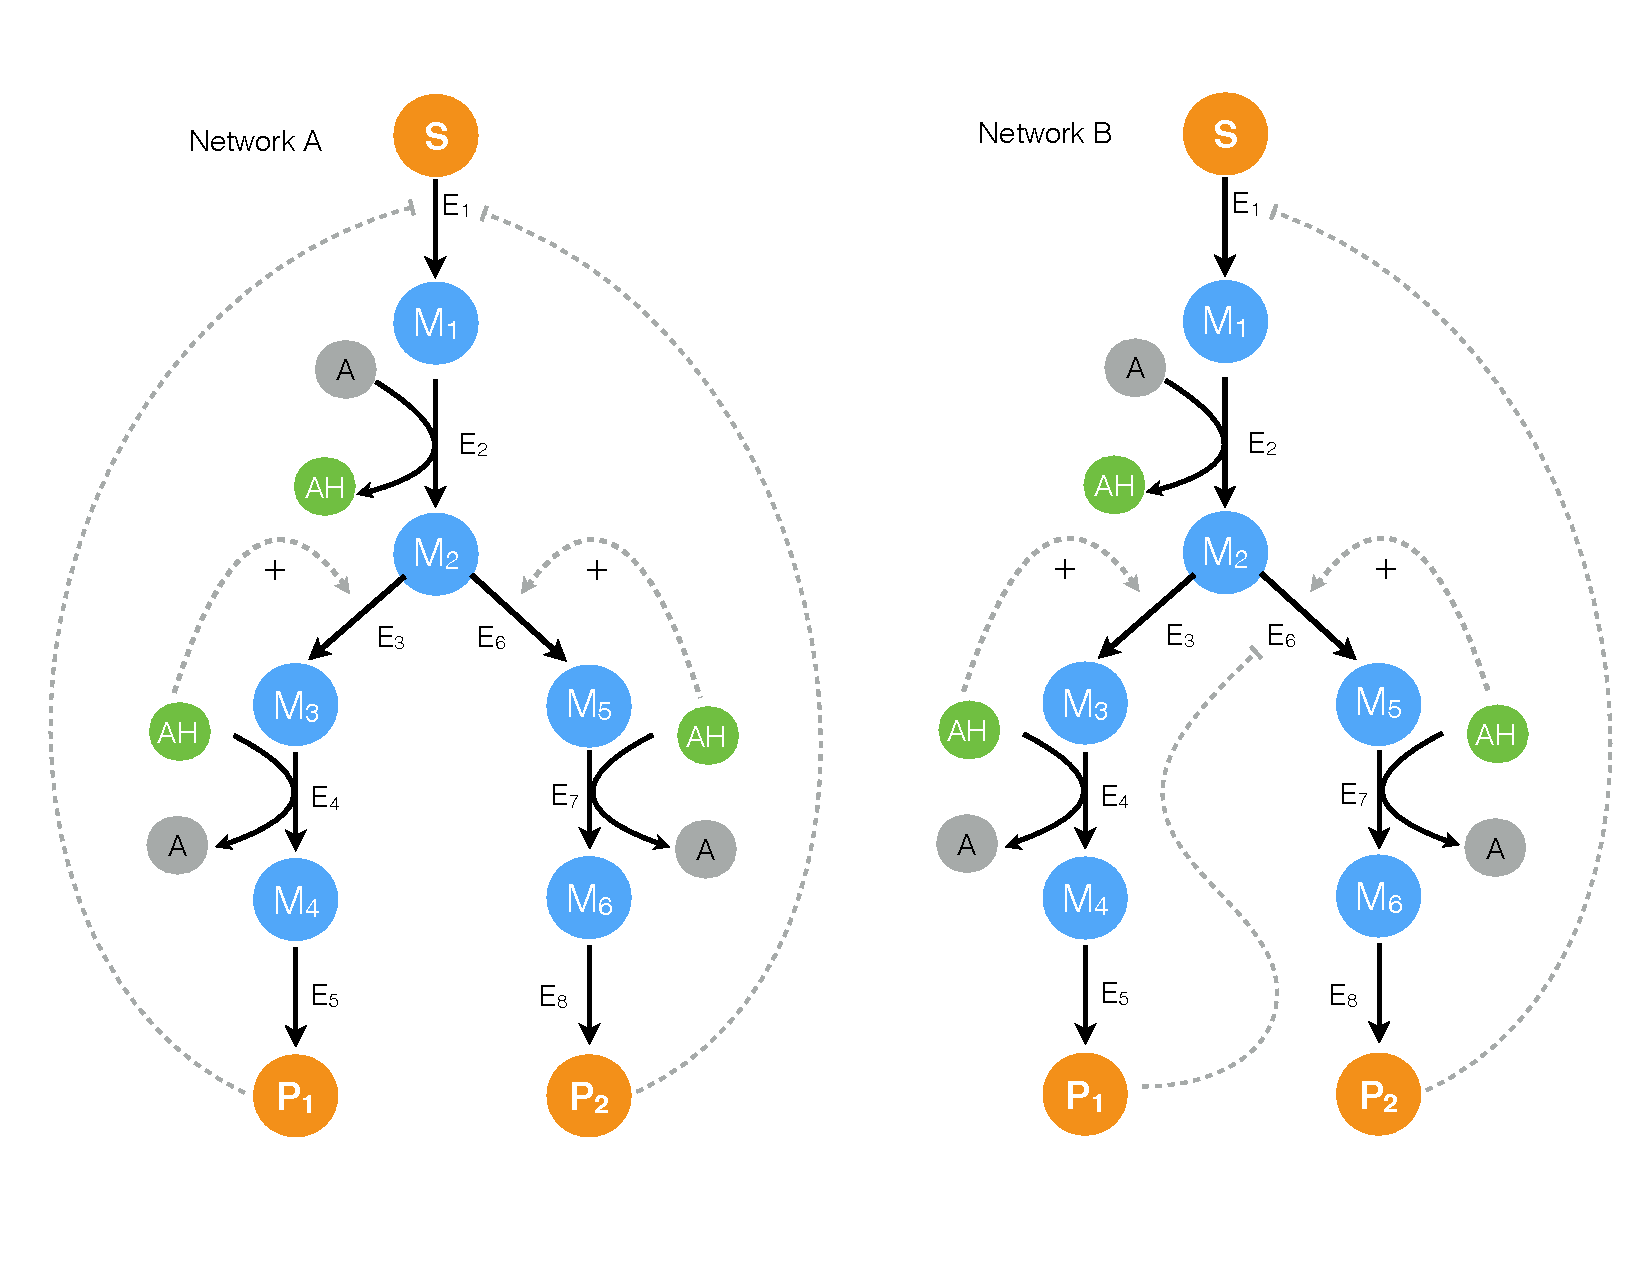
\includegraphics[width=1.0\textwidth]{./figs/Figure-1-Networks.pdf}
\caption{Proof-of-concept cell-free metabolic networks considered in this study. Substrate $S$ is converted to products P$_{1}$ and P$_{2}$ through a series of chemical conversions
catalyzed by enzyme(s) $E_{j}$. The activity of the pathway enzymes is subject to both positive and negative allosteric regulation. }\label{fig-networks}
\end{figure}

\clearpage

\begin{figure}
\centering
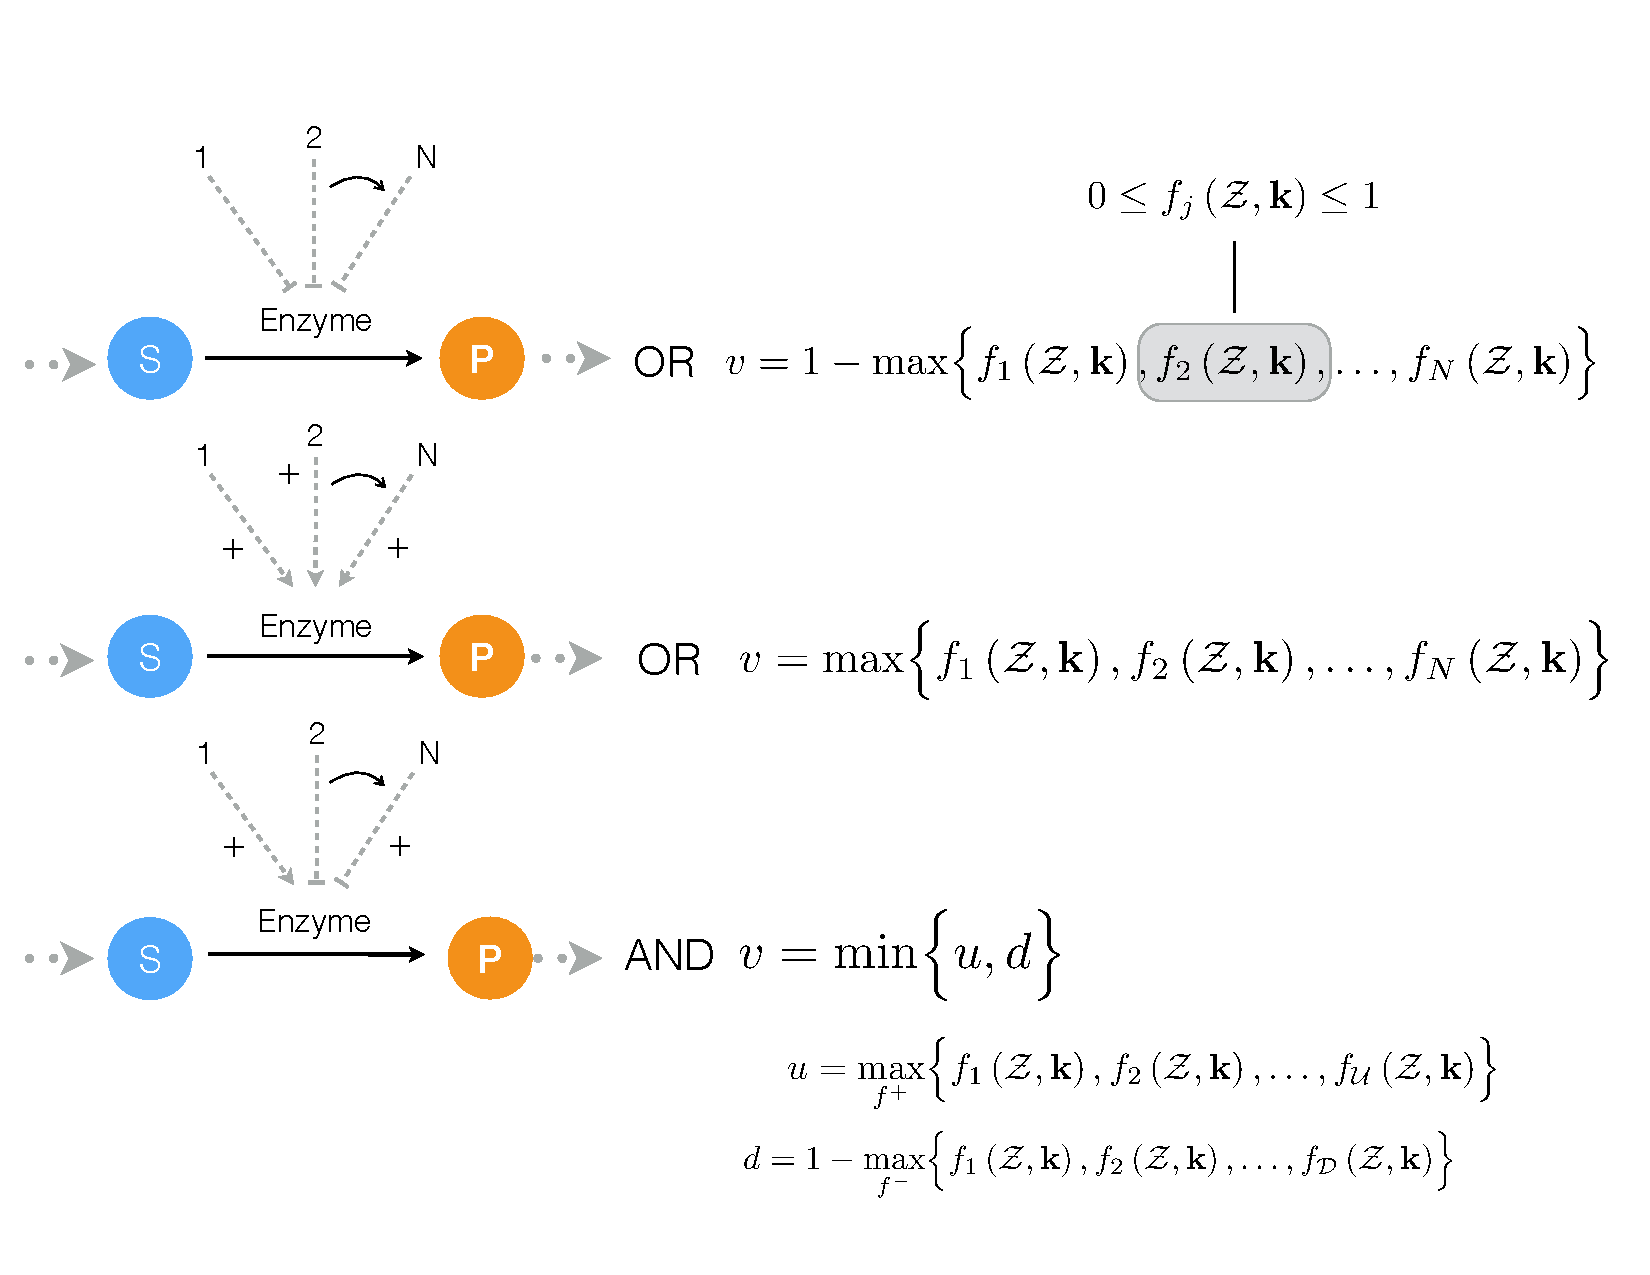
\includegraphics[width=1.0\textwidth]{./figs/Figure-2-ControlSchematic.pdf}
\caption{Schematic of rule-based allosteric enzyme activity control laws. 
Traditional enzyme kinetic expressions, e.g., Michaelis–Menten or multiple saturation kinetics, are multiplied by an enzyme activity control variable $0 \leq v_{j} \leq 1 $. 
Control variables are functions of many possible regulatory factors encoded by arbitrary functions of the form $0\leq f_{j}\left(\mathcal{Z}\right)\leq 1$.
At each simulation time step, the $v_{j}$ variables are calculated by evaluating integration rules such as the max or min of the set of factors $f_{1},\hdots$ 
influencing the activity of enzyme $E_{j}$. }\label{fig-control-schematic}
\end{figure}

\clearpage

\begin{figure}
\centering
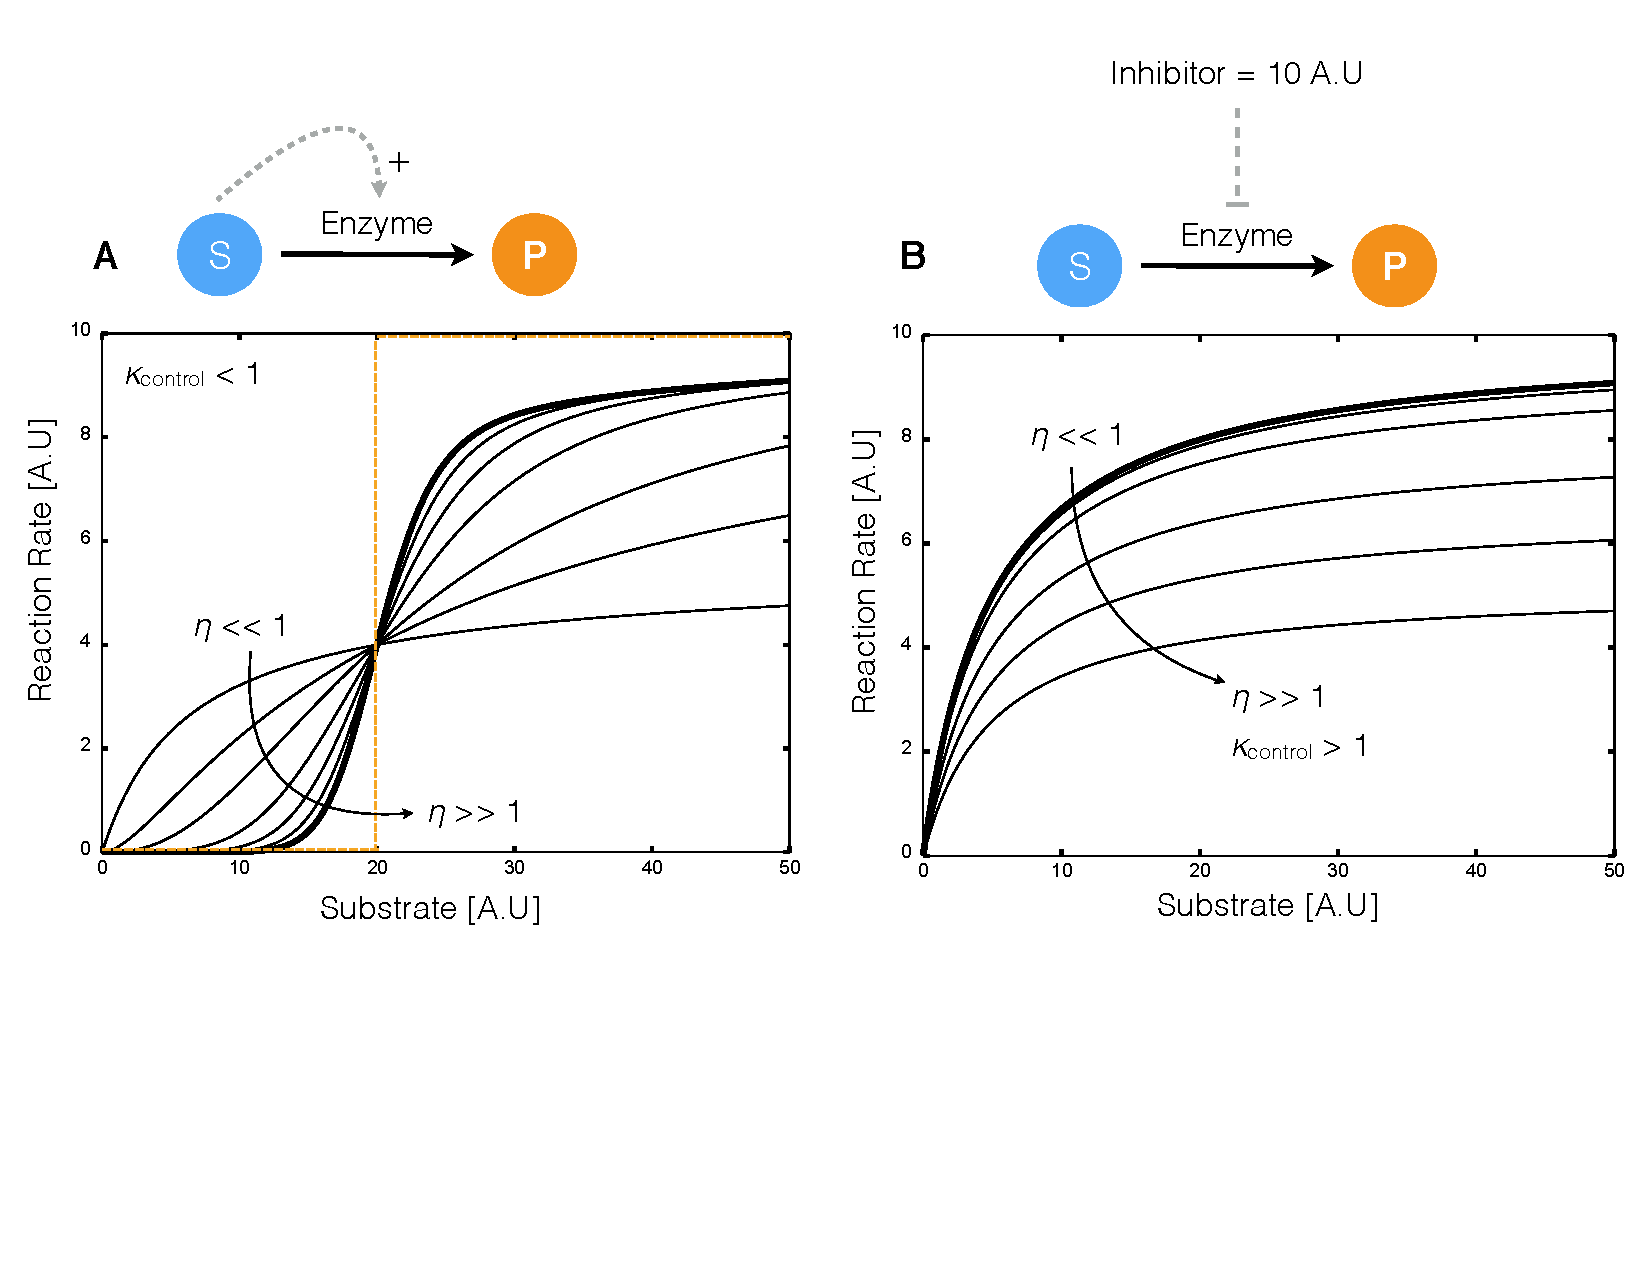
\includegraphics[width=1.0\textwidth]{./figs/Figure-3-EnzymeKinetics.pdf}
\caption{Kinetics of simple transformations in the presence of activation and inhibition. 
\textbf{A}:The conversion of substrate $S$ to product $P$ by enzyme $E$ was activated by $S$. 
For a fixed control gain parameter $\kappa_{control}$, the reaction rate approached a step for increasing cooperativity control parameter $\eta$. 
\textbf{B}:The conversion of substrate $S$ to product $P$ by enzyme $E$ with inhibitor $I$. 
For a fixed control gain parameter $\kappa_{control}$, the reaction rate approximated non-competitive inhibition for increasing cooperativity control parameter $\eta$. 
}\label{fig-kinetics-simulations}
\end{figure}

\clearpage

\begin{figure}
\centering
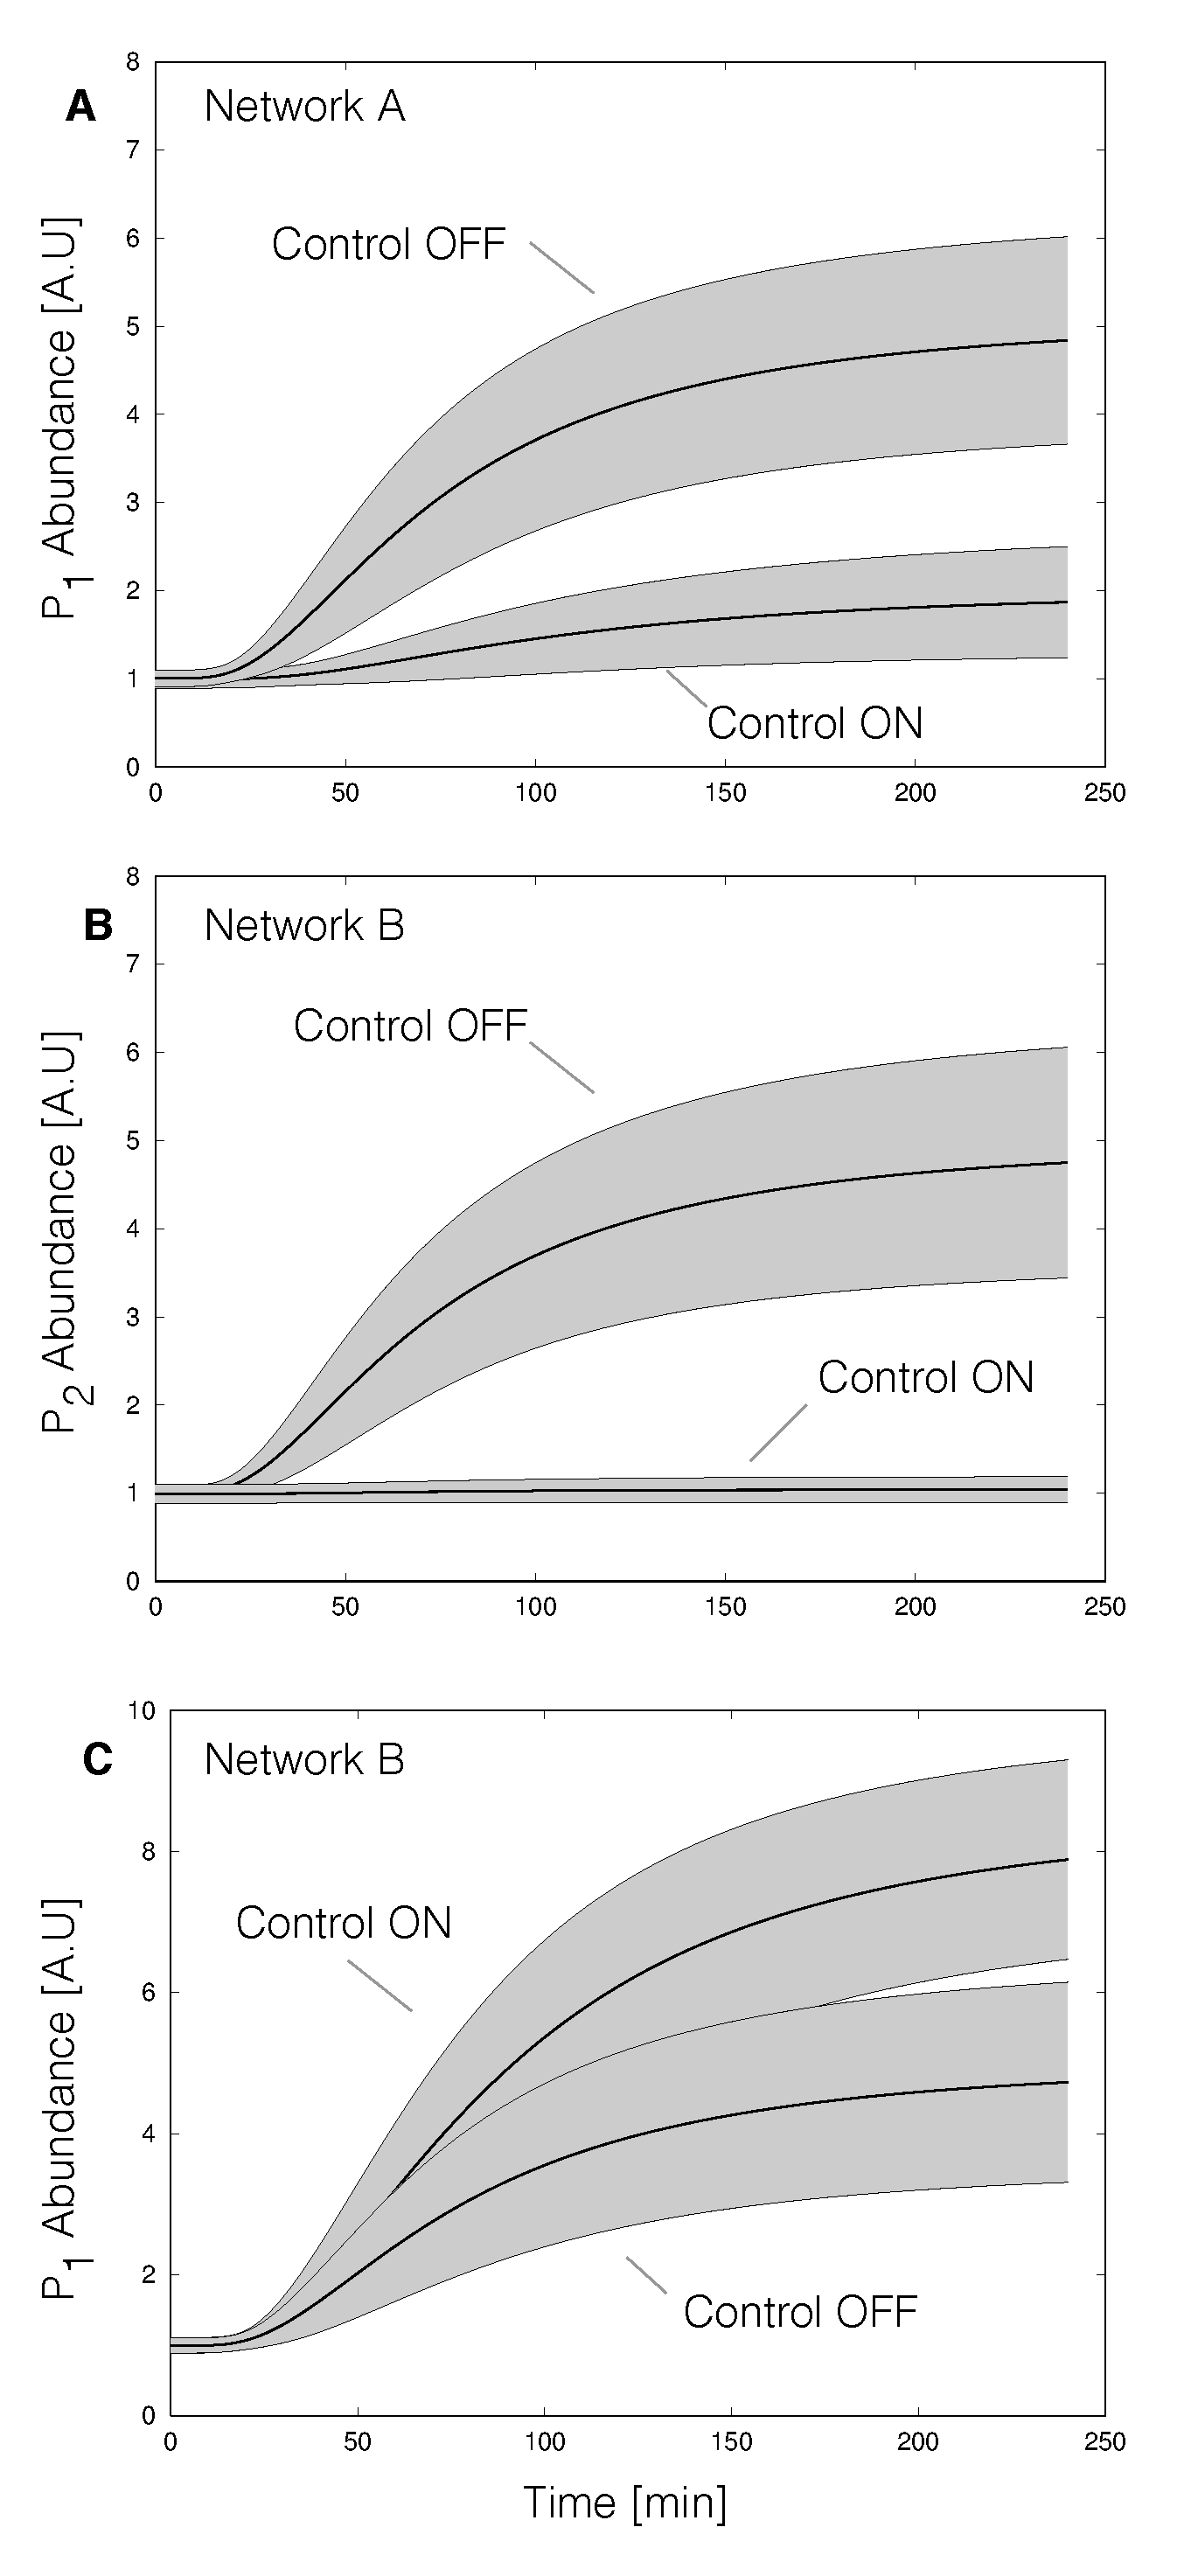
\includegraphics[width=0.50\textwidth]{./figs/Figure-4-OnOffSimulations.pdf}
\caption{ON/OFF control simulations for Network A and Network B for an ensemble of 100 kinetic parameter sets versus time. 
For each case, simulations were conducted using kinetic and initial conditions generated randomly from a hypothetical true parameter set. 
The gray area represents $\pm$ one standard deviation surrounding the mean. 
Control parameters were fixed during the ensemble calculations.
\textbf{A}: End product P$_{1}$ abundance versus time for Network A. 
The abundance of P$_{1}$ decreased with end product inhibition of $E_{1}$ activity (Control-ON) versus the no inhibition case (Control-OFF). 
\textbf{B}: End product P$_{2}$ abundance versus time for Network B. Inhibition of branch point $E_{6}$ by end product P$_{1}$ decreased P$_{2}$ abundance (Control-ON) versus the
no inhibition case (Control-OFF).
\textbf{C}: End product P$_{1}$ abundance versus time for Network A. 
Inhibition of branch point $E_{6}$ by end product P$_{1}$ decreased P$_{1}$ abundance (Control-ON) versus the no inhibition case (Control-OFF).
}\label{fig-onoff-simulations}
\end{figure}

\clearpage

\begin{figure}
\centering
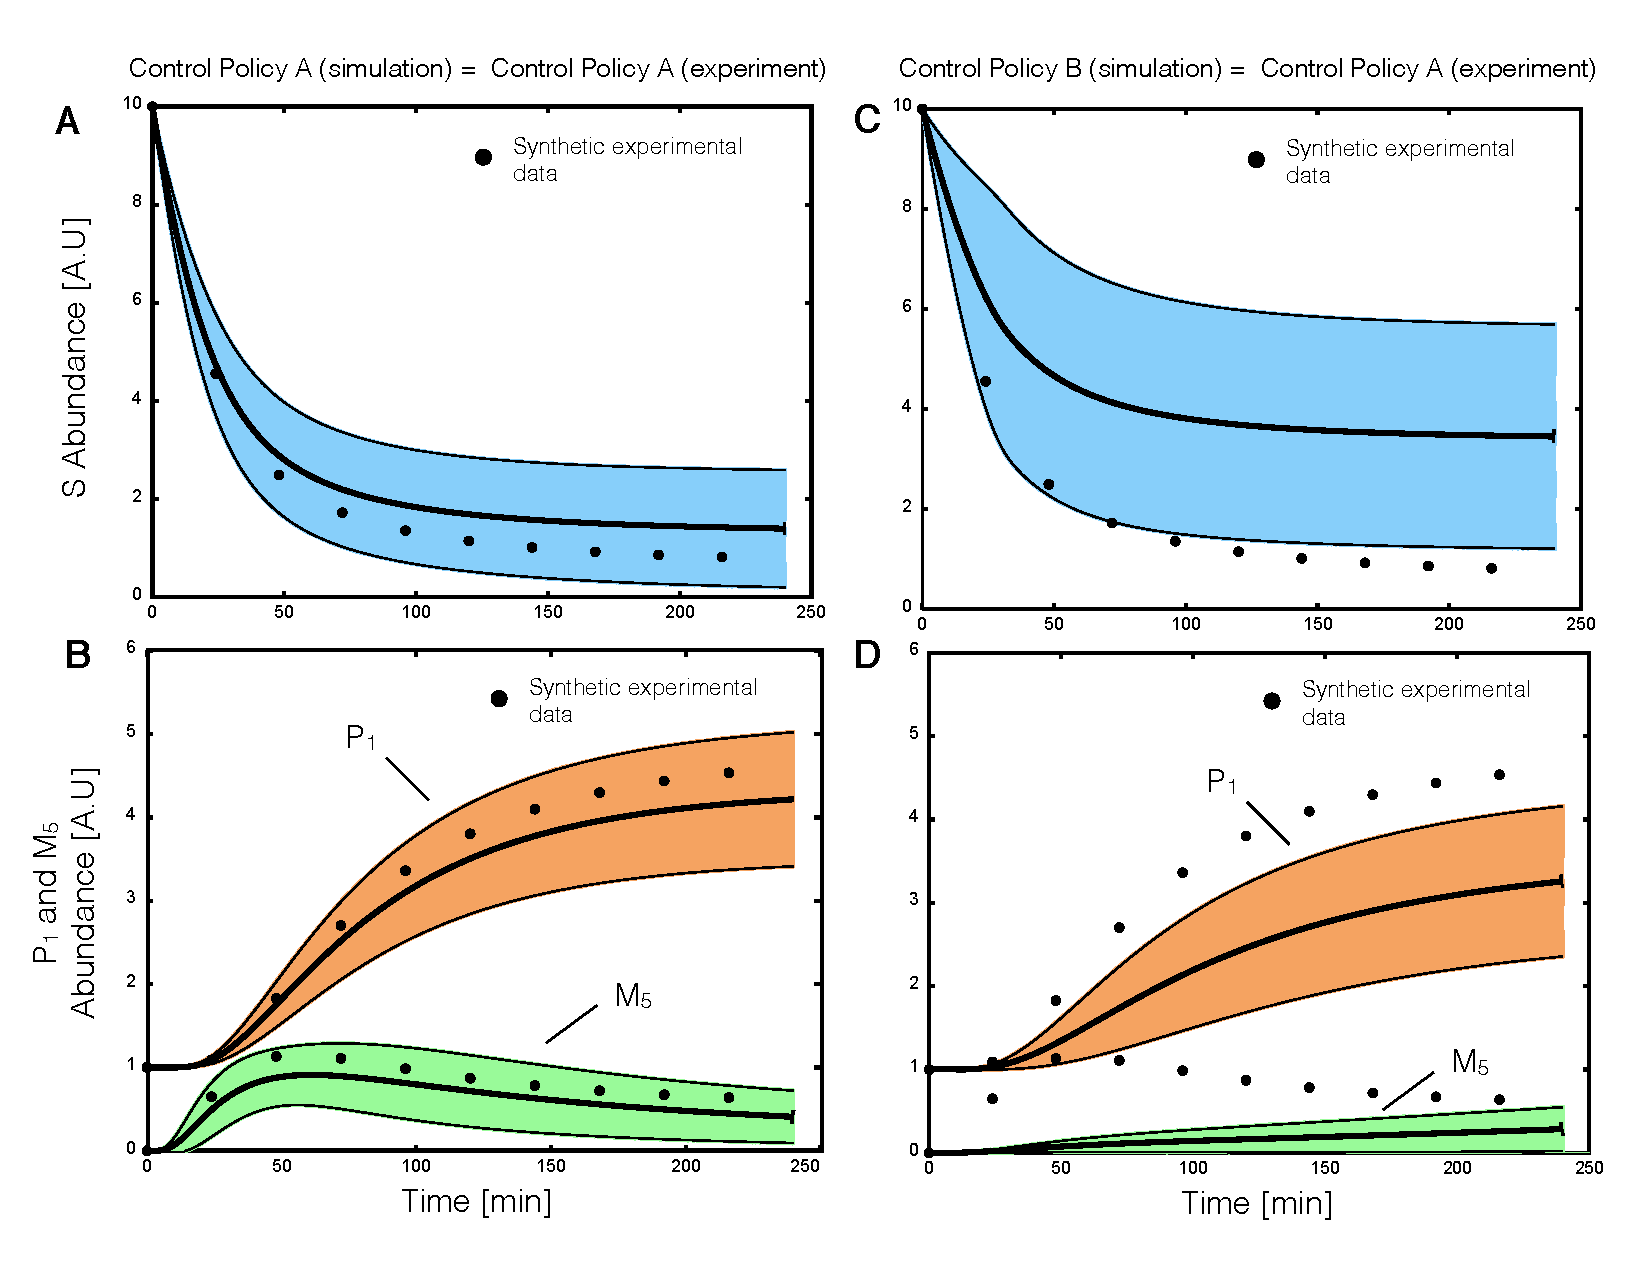
\includegraphics[width=1.0\textwidth]{./figs/Figure-5-ParameterFit.pdf}
\caption{Parameter estimation from synthetic data for the same and mismatched allosteric control logic using particle swarm optimization (PSO). 
Synthetic experimental data was generated from a hypothetical parameter set using Network A, 
where substrate $S$, end product P$_{1}$ and intermediate M$_5$ were sampled approximately every 20 minutes. 
For cases $\textbf{A,B}$ 20 particles were initialized with randomized parameters and allowed to search for 300 iterations. 
\textbf{A,B}: PSO estimated an ensemble of 20 parameters sets consistent with the synthetic experimental data assuming the correct
enzymatic and control connectivity starting from randomized initial parameters.
\textbf{C,D}: In the presence of control mismatch (Network B control policy simulated with Network A kinetic parameters) 
the ensemble of models did not describe the synthetic data. The synthetic data plotted here was unperturbed by noise. 
However, we assumed a coefficient of variation of 10\% for the synthetic data during parameter estimation.
}\label{fig-parameter-fit}
\end{figure}

\clearpage

\begin{figure}
\centering
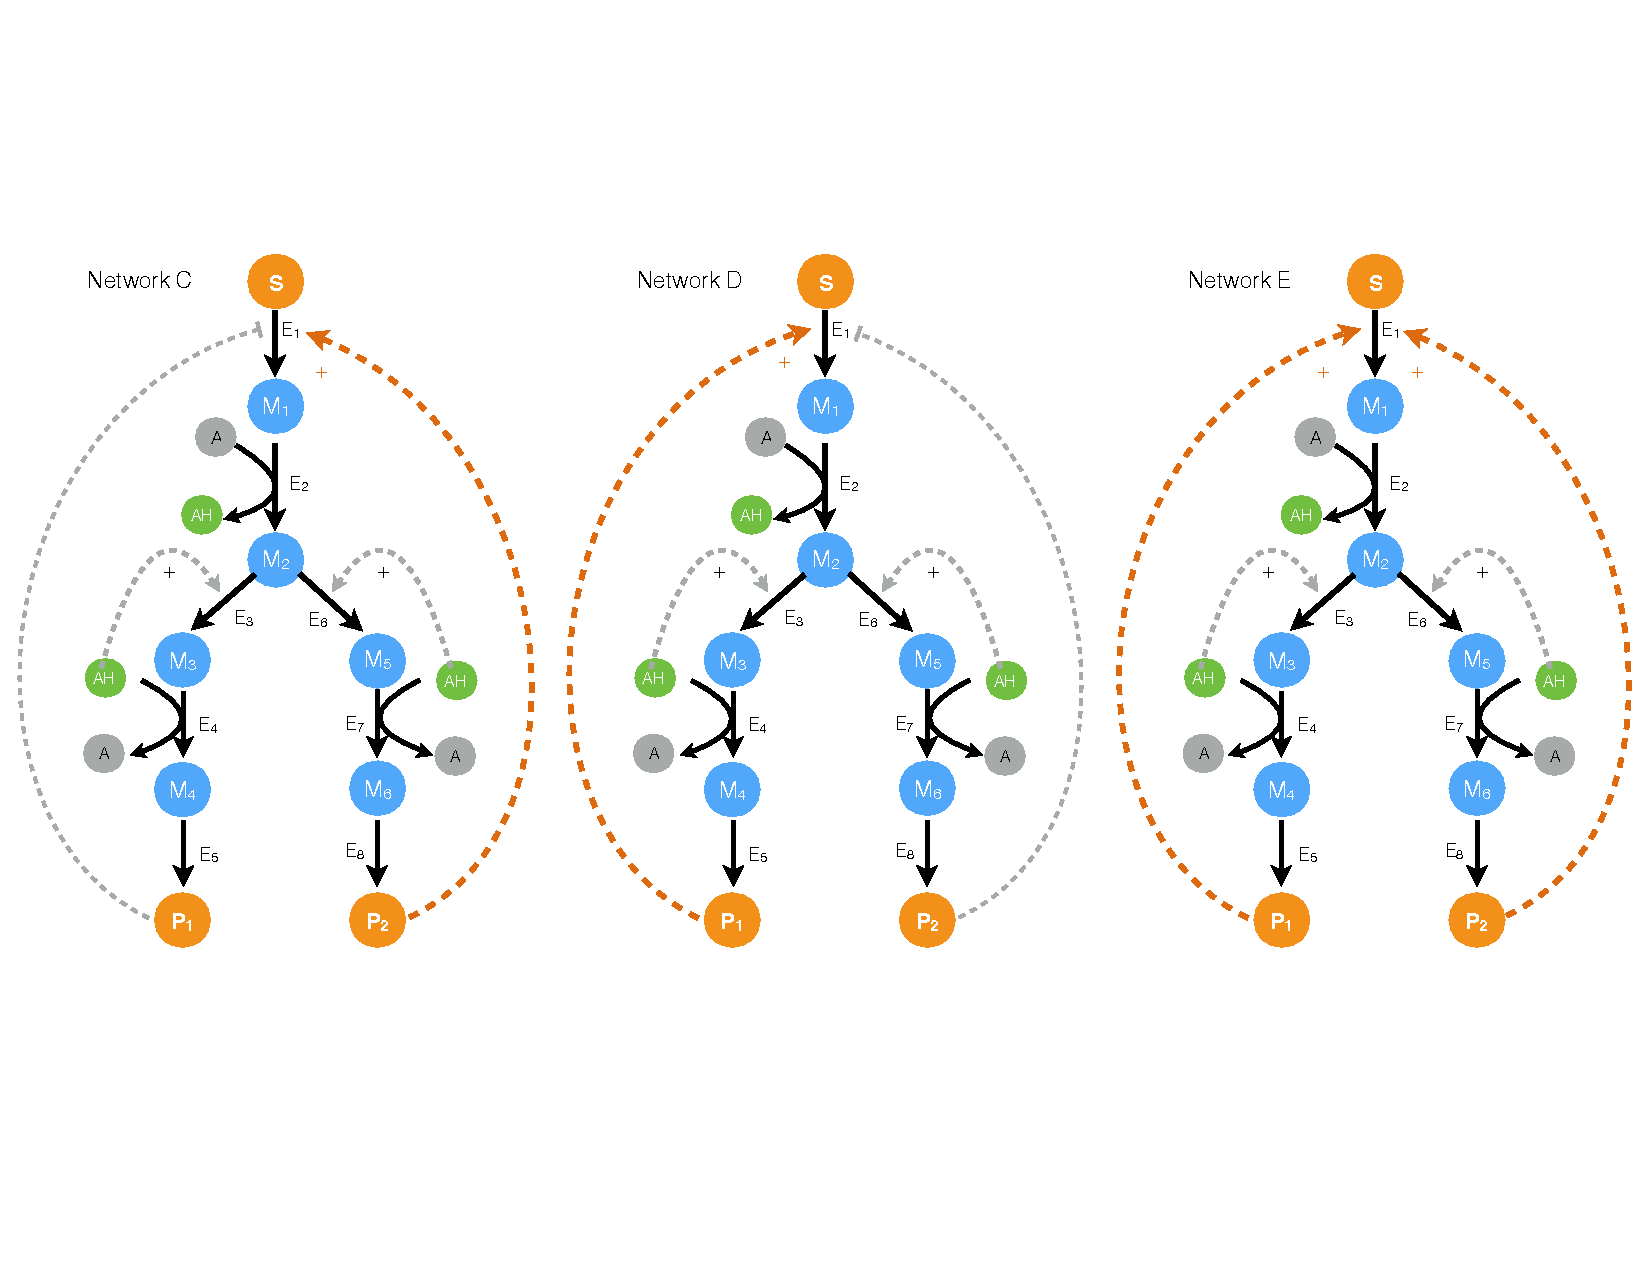
\includegraphics[width=1.0\textwidth]{./figs/Figure-6-AlternativeNetworks.pdf}
\caption{Schematic of the alternative allosteric control programs used in the structural particle swarm computation. 
Each network had the same enzymatic connectivity, initial conditions and kinetic parameters, 
but alternative feedback control structures for the first enzyme in the pathway.}\label{fig-alternative-networks}
\end{figure}

\clearpage

\begin{figure}
\centering
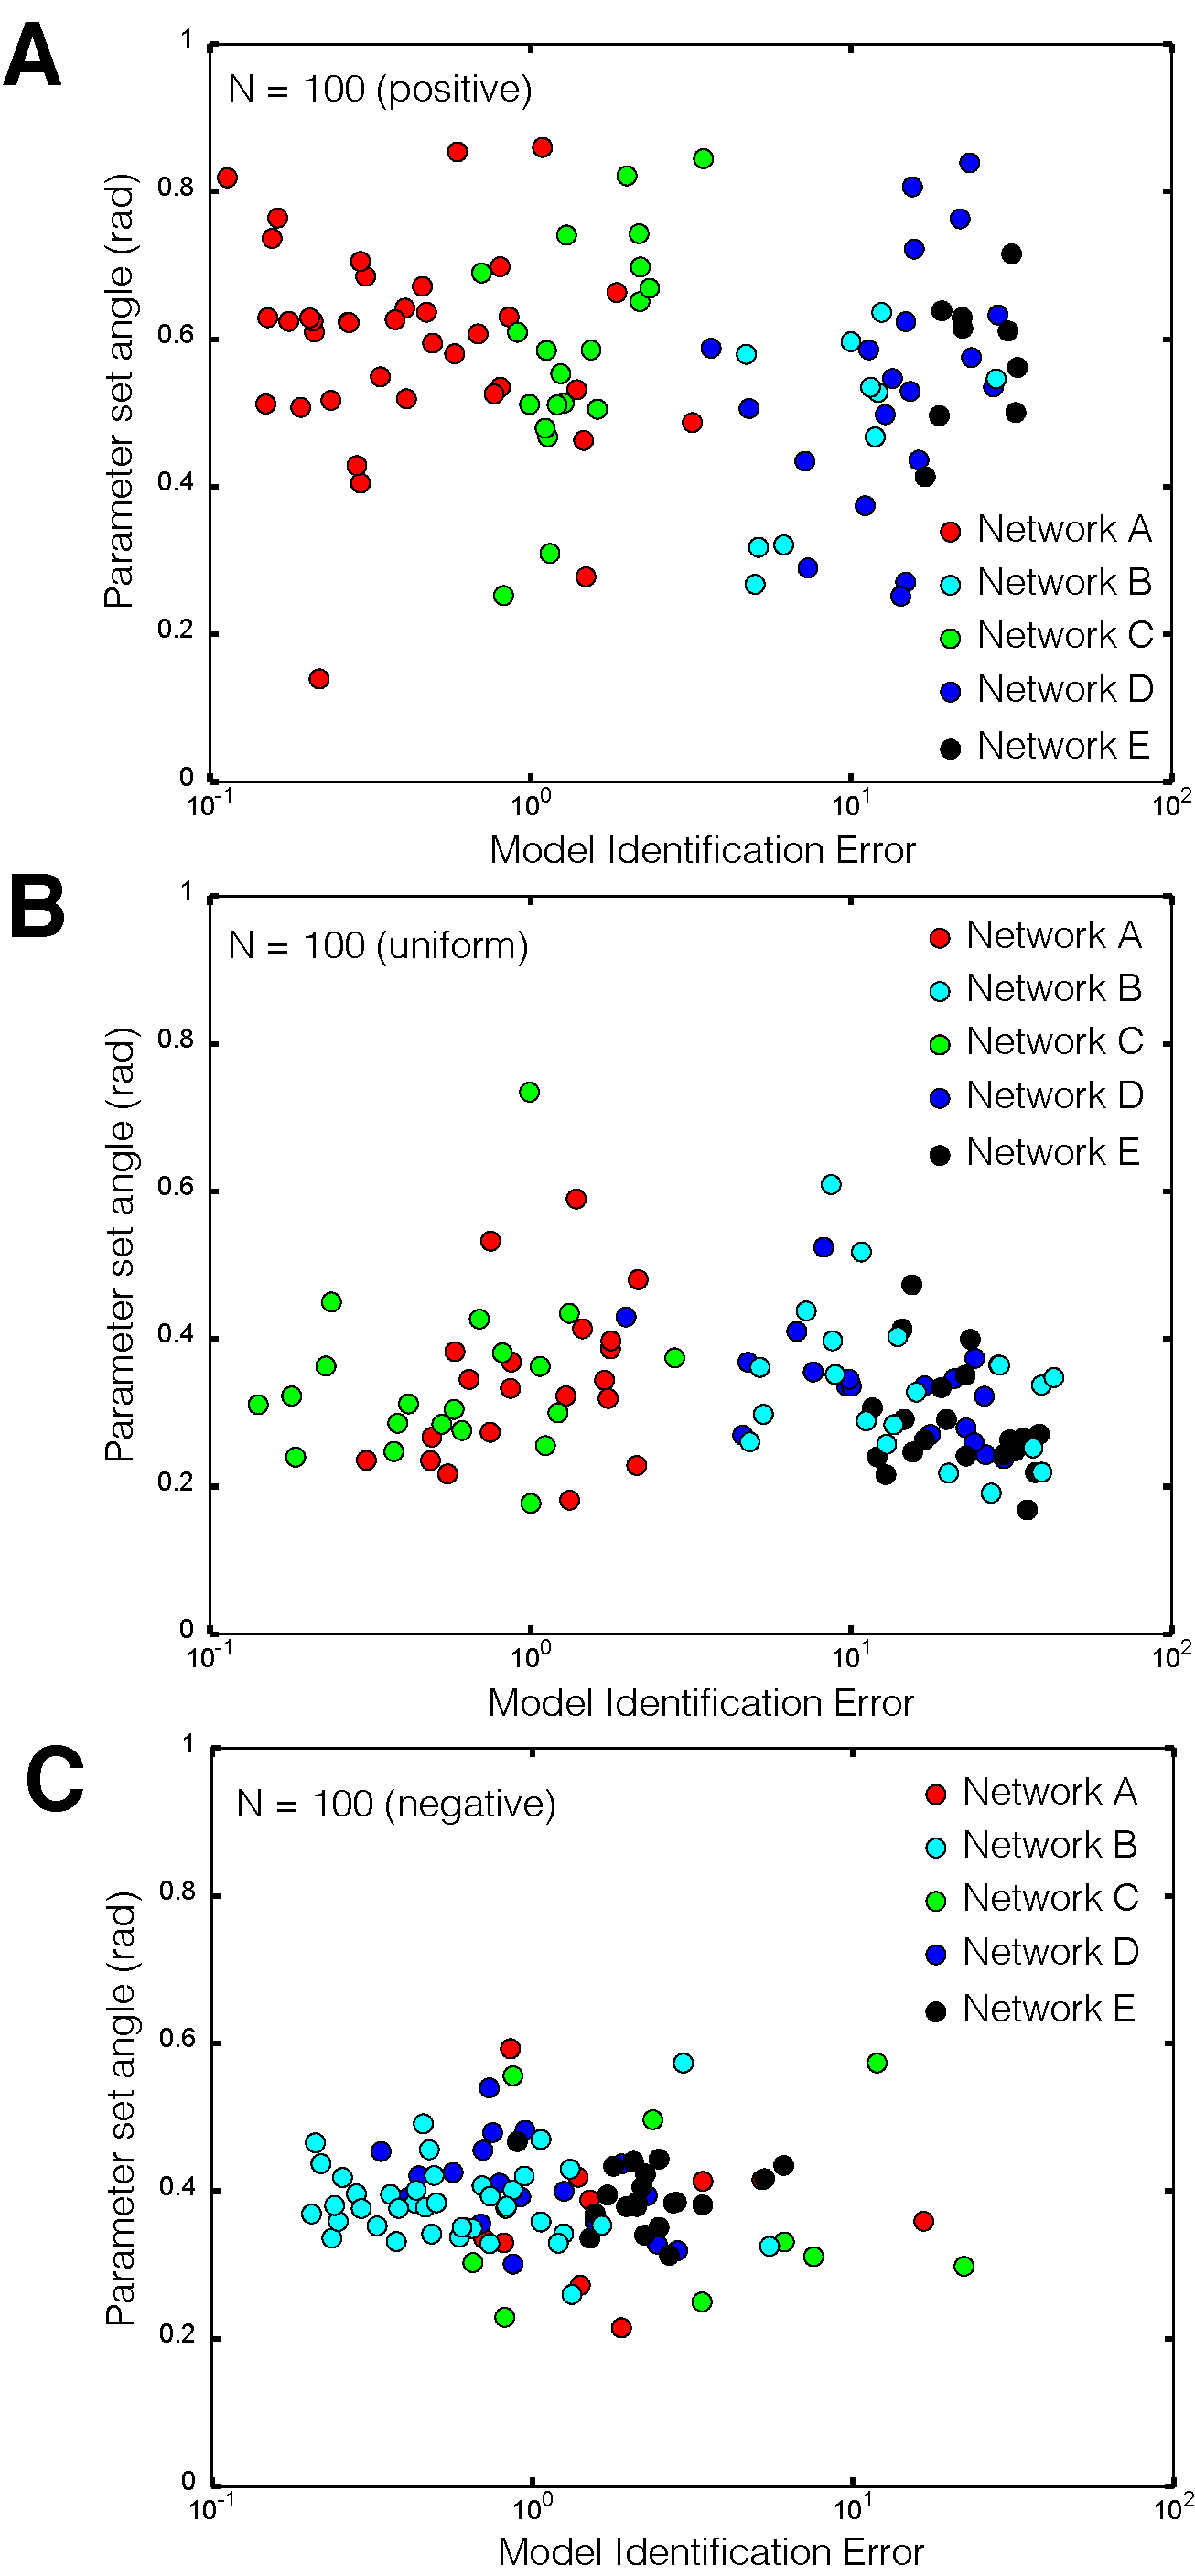
\includegraphics[width=0.5\textwidth]{./figs/Figure-7-ControlSearch.pdf}
\caption{Combined control and kinetic parameter search using modified particle swarm optimization (PSO). 
A population of 100 particles was initialized with randomized kinetic parameters and one of five possible control configurations (Network A - E).
Simulation error was minimized for a synthetic data set 
($S$, end product P$_{1}$ and intermediate M$_5$ sampled approximately every 20 min) generated using Network A.
\textbf{A}: Simulation error versus parameter set angle for 100 particles biased toward the correct regulatory program (A,B,C,D,E) = (40\%, 10\%, 20\%, 20\% and 10\%).
\textbf{B}: Simulation error versus parameter set angle for 100 uniformly distributed particles (A,B,C,D,E) = (20\%, 20\%, 20\%, 20\% and 20\%).
\textbf{C}: Simulation error versus parameter set angle for 100 negatively biased particles (A,B,C,D,E) = (10\%, 40\%, 10\%, 20\% and 20\%).
Network A (the correct structure) was preferentially identified for positively and uniform biased particle distributions, but misidentified in the presence of
a large incorrect bias. 
}\label{fig-control-search}
\end{figure}

\clearpage

\begin{figure}
\centering
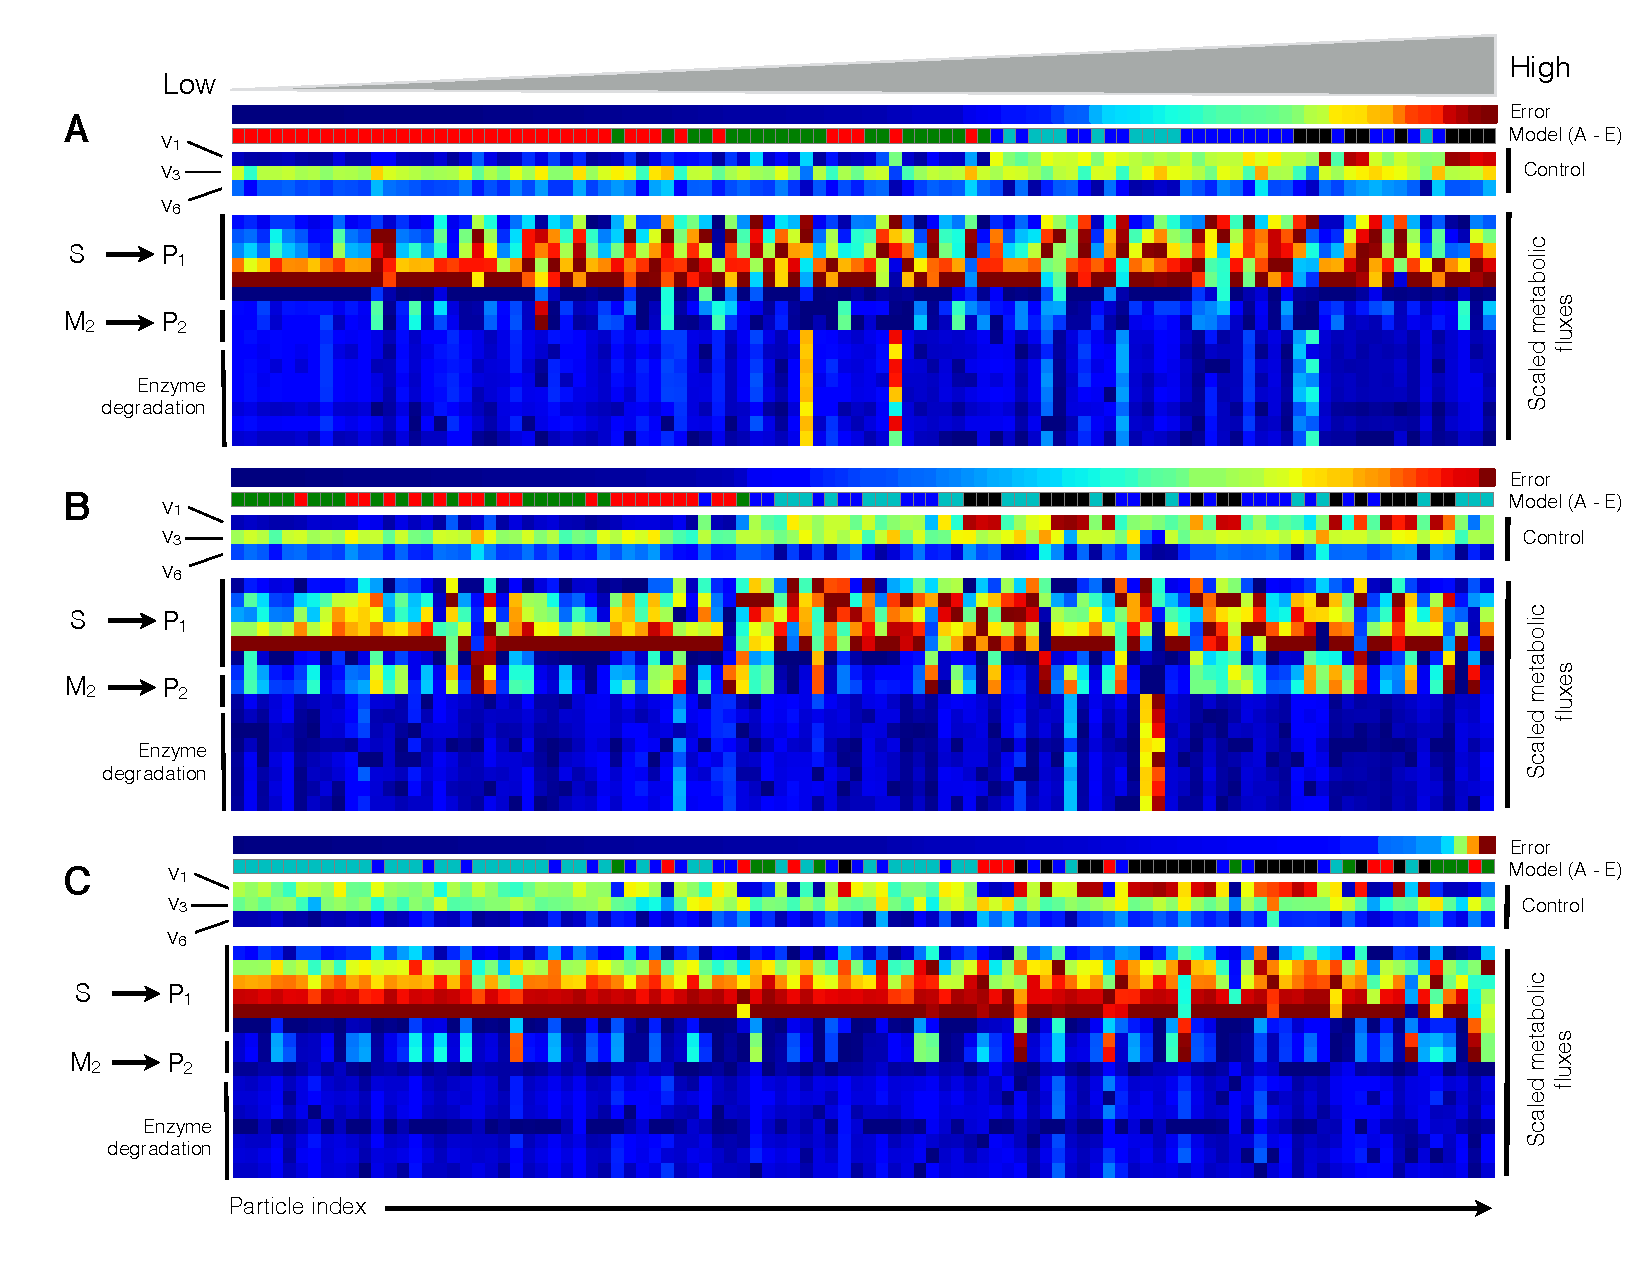
\includegraphics[width=1.0\textwidth,height=0.6\textheight]{./figs/Figure-8-Flux.pdf}
\caption{Metabolic flux and control variables as a function of network type and particle index at t = 100 min.
The control variables governing $E_{1},E_{3}$ and $E_{6}$ activity and the scaled metabolic flux were calculated for the positively (top), 
uniformly (middle) and negatively (bottom) biased particle swarms (N = 100). 
Blue denotes a low value, while red denotes a high value for the respective quantity being plotted.
The particles from each swarm were sorted based upon simulation error (low to high error). 
\textbf{A}: Model performance for the positively biased particle swarm as a function of particle index.
\textbf{B}: Model performance for the uniformly biased particle swarm as a function of particle index.
\textbf{C}: Model performance for the negatively biased particle swarm as a function of particle index. 
Models with significant control mismatch showed distinct control and flux patterns versus those models with the correct or closely related control policies.
In particular, models with the correct control policy showed stronger inhibition of $E_{1}$ activity, leading to decreased flux from S$\rightarrow$P$_{1}$.
Conversely, models with significant mismatch had increased $E_{1}$ activity, leading to an altered flux distribution. 
This is especially apparent in the negatively biased particle swarm. 
}\label{fig-flux-pattern}
\end{figure}

\clearpage

% Supplemental figures -
% Set the S- 
\renewcommand\thefigure{S\arabic{figure}}
\renewcommand\thetable{T\arabic{table}}
\renewcommand\thepage{S-\arabic{page}}
\renewcommand\theequation{S\arabic{equation}}

% Reset the counters -
\setcounter{equation}{0}
\setcounter{table}{0}
\setcounter{figure}{0}
\setcounter{page}{1}

\end{document}

